\documentclass[../DoAn.tex]{subfiles}
\begin{document}
\raggedbottom
Trong chương này, em sẽ thực hiện khảo sát một số hệ thống cũng như người dùng, từ đó phân tích các use case quan trọng của hệ thống đồng thời đề ra một số yêu cầu phi chức năng.
\section{Khảo sát hiện trạng}
\label{section:2.1}
Ở phần này trước hết ta sẽ tìm hiểu về hai thuật ngữ là hệ thống theo dõi ứng viên (ATS) và hệ thống quản lý nguồn nhân lực (HRIS). Hệ thống theo dõi ứng viên được xem như là một công cụ rất cần thiết cho quy trình tuyển dụng, cho phép quản lý các đầu việc từ đăng tuyển công việc cho đến ứng tuyển và thông báo trạng thái đỗ hay trượt của ứng viên. Nhìn chung, ATS giúp theo dõi toàn bộ hoạt động của quy trình tuyển dụng, có thể giúp tiết kiệm đáng kể thời gian và công sức. Trong khi đó hệ thống quản lý nguồn nhân lực hướng đến quản lý các thông tin của những nhân viên của công ty như là thông tin hồ sơ, quá trình đào tạo, lương thưởng, chấm công,...Vì đều là các hệ thống liên quan đến quản lý nguồn nhân lực nên ATS và HRIS có sự bổ trợ lẫn nhau. Nếu tận dụng tốt sức mạnh của các hệ thống này thì quản lý nguồn nhân lực sẽ đạt hiệu quả rất cao.

Như đã đề cập, ATS và HRIS có thể dùng bổ trợ lẫn nhau nên hiện nay đã xuất hiện những hệ thống kết hợp, vừa giúp quản lý quy trình tuyển dụng vừa hỗ trợ quản lý nhân sự của công ty. Sự kết hợp này đem đến nhiều lợi ích như:
\begin{itemize}
\item Có một cái nhìn tổng quan về toàn bộ nguồn nhân lực của công ty
\item Quản lý tập trung, chia sẻ dữ liệu dùng chung
\item Chỉ cần một trang web cho cả hai mục tiêu, từ đó nâng cao trải nghiệm sử dụng bởi sự liền mạch
\item Hiệu quả trong thống kê, phân tích và báo cáo
\end{itemize}

\subsection{Khảo sát một số hệ thống}
Trước hết, DATN thực hiện khảo sát các hệ thống hiện có. Với mong muốn tạo ra một ứng dụng "kết hợp" cả ATS và HRIS nên DATN chỉ khảo sát các hệ thống tương tự như vậy. Như đã đề cập từ các phần trước, các hệ thống kiểu vậy chưa xuất hiện nhiều, ở đây sẽ khảo sát qua ba hệ thống bao gồm: Deel, Paycor và Eddy.

\subsubsection{Deel}\cite{Deel}
Theo như mô tả ở trang chủ của Deel, đây là một sản phẩm giúp quản lý toàn bộ nguồn nhân lực của công ty từ nhân viên trực tiếp đến nhân viên quốc tế và mọi thứ ở giữa nữa. Deel có thể sử dụng cho các công ty cỡ từ lớn đến nhỏ và hỗ trợ duy nhất nền tảng web. Deel cung cấp các tính năng hỗ trợ chủ yếu cho quản lý nhân viên trong công ty, với sự tin tưởng từ những công ty nổi tiếng như Dropbox, LG, Cloudflare và Shopify. Phần dưới đây nêu ra một số ưu và nhược điểm của nền tảng này:

\textbf{Ưu điểm}
\begin{itemize}
    \item Hỗ trợ đa dạng các tính năng trên mọi khía cạnh của quản lý nhân sự
    \item Tính năng quản lý trả lương và quản lý đãi ngộ được nhiều người sử dụng yêu thích
    \item Cung cấp tính ký kết và thuê các nhân viên từ mọi nơi trên thế giới một cách hợp pháp
    \item Quản lý hồ sơ nhân viên và các yêu cầu của nhân viên (như nghỉ phép, nghỉ ốm,...)
    \item Đối với việc quản lý nhân sự không phải là nhân viên của công ty, Deel phát triển tính năng quản lý tài năng
    \item Bố trí giao diện tương đối dễ sử dụng
    \item Và nhiều tính năng khác
\end{itemize}

\textbf{Nhược điểm}
\begin{itemize}
    \item Chưa hỗ trợ tính năng tạo và làm bài kiểm tra online cho ứng viên
    \item Mức giá khởi điểm khá cao với 49 đô một tháng và trên một người sử dụng
    \item Chưa có tính năng đánh giá ứng viên
    \item Cài đặt ứng dụng đôi khi gặp khó khăn bởi vì ở nhiều tình huống Deel chưa có các hướng dẫn cụ thể
    \item Chưa có tính năng quản lý sự có mặt của nhân viên ở công ty
    \item Chưa có tính năng quản lý chương trình đào tạo
\end{itemize}

\subsubsection{Paycor}\cite{Paycor}
Paycor là một hệ thống hỗ trợ đơn giản hóa công việc của bộ phận nhân sự bởi mọi thông tin cần thiết được tập trung trong một hệ thống. Paycor cũng cung cấp nhiều tính năng tự động, từ đó giúp tiết kiệm tối đa thời gian. Cũng như Deel, Paycor giúp tuyển dụng nhân viên từ các nơi trên thế giới một cách hợp pháp. Một số tổ chức dùng Paycor có thể kể đến là Toronto Transit Commission, Meta Platforms, Blackfriars Group.

\textbf{Ưu điểm}
\begin{itemize}
    \item Cung cấp tính năng theo dõi ứng viên và đánh giá ứng viên
    \item Có tính năng chat nội bộ
    \item Tính năng thông báo trong thời gian thực giúp cho bộ phận nhân sự nắm bắt được mọi sự kiện một cách nhanh chóng nhất
    \item Phát triển tính năng thu hút tài năng giúp công ty luôn có nguồn nhân sự chất lượng cao
    \item Quản lý hồ sơ nhân viên và các yêu cầu của nhân viên (như nghỉ phép, nghỉ ốm,...)
    \item Hỗ trợ giao diện trên cả máy tính bảng và điện thoại
    \item Và nhiều tính năng khác
\end{itemize}

\textbf{Nhược điểm}
\begin{itemize}
    \item Chưa hỗ trợ tính năng tạo và làm bài kiểm tra online cho ứng viên
    \item Chưa có tính năng quản lý chương trình đào tạo
    \item Mức giá khởi điểm rất cao từ 99 đô la một tháng và đây có lẽ là nhược điểm lớn nhất của Paycor
    \item Giao diện chưa được thân thiện với người sử dụng
\end{itemize}

\subsubsection{Eddy}\cite{Eddy}
Ngay khi truy cập trang chủ của Eddy, người dùng sẽ thấy dòng chia sẻ rằng Eddy là một sản phẩm dành cho bộ phận nhân sự với tất cả các tính năng trong chỉ một hệ thống, hỗ trợ tuyển dụng, quản lý, trả lương nhân viên một cách dễ dàng mà không phải chịu bất cứ cảnh đau đầu nào. Eddy là một ứng dụng trả phí với khởi diểm 8 đô la trên một tháng và có thể sử dụng cho nhiều kiểu user như doanh nghiệp từ lớn đến nhỏ, tổ chức phi lợi nhuận, hành chính công. Eddy cung cấp một loạt các tính năng hỗ trợ gần như tất cả mọi thứ liên quan đến tuyển dụng và nhân sự của công ty, tổ chức. Tuy nhiên ứng dụng nào cũng có những ưu điểm và nhược điểm. Với Eddy, những ưu nhược điểm có thể kể đến như là:

\textbf{Ưu điểm}
\begin{itemize}
    \item Cách bố trí rất đơn giản nhưng tiện lợi, dễ sử dụng và giúp người dùng tập trung vào công việc chính
    \item Cung cấp tính năng tạo công việc, theo dõi ứng viên hỗ trợ tốt cho bộ phận tuyển dụng của công ty
    \item Cung cấp tính năng theo dõi thời gian giúp cho người dùng kiểm soát được tiến trình của mọi công việc, đây là một trong những tính năng được rất nhiều người dùng yêu thích khi sử dụng Eddy
    \item Hỗ trợ lưu trữ các tài liệu quan trọng của công ty
    \item Quản lý hồ sơ nhân viên và các yêu cầu của nhân viên (như nghỉ phép, nghỉ ốm,...)
\end{itemize}

\textbf{Nhược điểm}
\begin{itemize}
    \item Chưa hỗ trợ tính năng tạo và làm bài kiểm tra online cho ứng viên
     \item Chưa có tính năng quản lý chương trình đào tạo
    \item Chưa hỗ trợ thông báo trong thời gian thực
    \item Có nhiều tính năng tuy đã công bố nhưng chưa được phát triển và đưa vào sử dụng
\end{itemize}

\subsection{Khảo sát nhu cầu của một số công ty}
Tiếp theo, em thực hiện khảo sát nhu cầu quản lý nhân sự của một số công ty thông qua một số người hiện là nhân viên của các công ty đó.

Bạn Thái Doãn Đạt hiện là nhân viên của một công ty có khoảng 60 người. Hiện công ty chưa sử dụng hệ thống tích hợp ATS và HRIS nào vì số lượng nhân viên không quá lớn và các hệ thống như vậy thường có mức giá cao trong khi nhu cầu của công ty không cần thiết sử dụng hết chức năng của các hệ thống ấy, nên bộ phận nhân sự thông thường sẽ đăng các tin tuyển dụng thông qua mạng xã hội và ứng viên sẽ liên hệ với công ty thông qua các thông tin ở những bài đăng ấy. Hiện tại công ty cũng chưa có trang web hay hệ thống nào giúp ứng viên tìm hiểu về các việc làm cũng như cơ hội phát triển của công ty. Vì vậy, công ty cũng có nhu cầu tìm một ứng dụng có thể giúp ứng viên tìm hiểu về công ty, về môi trường và cơ hội việc làm, giúp bộ phận nhân sự đăng các tin tuyển dụng và trao đổi với ứng viên mà không cần thông qua các mạng xã hội, có thể kiểm tra sơ bộ năng lực của nhân viên bằng hình thức online, đồng thời giúp công ty quản lý được các hoạt động diễn ra hằng ngày xung quanh chủ thể chính là các nhân viên. 

Bạn Vương Văn Trường hiện là nhân viên của một công ty có hơn 150 người. Với số lượng nhân viên nhiều như vậy, công ty đã phát triển một ứng dụng để tiện cho việc quản lý nhân viên trong công ty. Về vấn đề tuyển dụng công ty cũng phát triển một hệ thống tách biệt giúp ứng viên tìm hiểu về công ty và các cơ hội việc làm. Công ty cũng có nhu cầu chỉ cần một hệ thống mà có thể giải quyết được cả hai mục tiêu chính là tuyển dụng và quản lý nhân viên. Đồng thời hệ thống cũng giúp đánh giá ứng viên online trước khi bước tới những khâu tiếp theo của quy trình tuyển dụng. 

Sau khi khảo sát các hệ thống ở trên cũng như khảo sát nhu cầu của một số công ty, em thấy rằng những tính năng dưới đây là cần thiết cho một hệ thống hỗ trợ tuyển dụng và quản lý nhân sự:

\begin{itemize}
\item \textbf{Tìm kiếm việc làm:} Tính năng này giúp người dùng tìm kiếm các công việc mà công ty đang cần tuyển nhân sự
\item \textbf{Nộp đơn ứng tuyển:} Tính năng này giúp các ứng viên gửi đơn ứng tuyển về hệ thống và bắt đầu cho một "phiên" tuyển dụng
\item \textbf{Quản lý các công việc cần tuyển:} Đây là thông tin hữu ích đối với các ứng viên, nhờ đó ứng viên hiểu được phần nào về nhu cầu nhân lực của công ty, hiểu sơ bộ về yêu cầu đối với công việc mà ứng viên đang quan tâm cũng như cơ hội phát triển của bản thân
\item \textbf{Làm bài kiểm tra kỹ năng:} Tính năng này là như là một bước bắt buộc của quá trình tuyển dụng. Qua một bài kiểm tra năng lực sơ bộ, bộ phận tuyển dụng của công ty phần nào đánh giá được năng lực và tư duy của ứng viên
\item \textbf{Quản lý hồ sơ ứng viên:} Đây là một tính năng quan trọng, nhờ có dữ liệu của ứng viên ta có thể khai thác thêm nhiều thông tin, và các dữ liệu đó cũng chính là đầu vào của nhiều tính năng khác
\item \textbf{Quản lý hồ sơ nhân viên:} Tương tự như phần quản lý hồ sơ ứng viên, dữ liệu nhân viên là quan trọng nhất vì mọi hoạt động của hệ thống quản lý nhân sự đều xoay quanh các nhân viên
\item \textbf{Quản lý chấm công:} Đây là tính năng cần có của một hệ thống quản lý nhân sự HRIS. Tính năng này cho phép theo dõi hoạt động của nhân viên tại công ty từ thời gian bắt đầu và kết thúc một ngày làm việc, các yêu cầu xin nghỉ hay xin làm từ xa,...
\item \textbf{Quản lý các chương trình đào tạo:} Nhận thấy rằng việc đào tạo nhân lực để nguồn nhân lực ngày càng chất lượng hơn là cần thiết. Tính năng này cho phép các nhân viên theo dõi và tham gia các chương trình đào tạo của công ty, giúp bộ phận quản lý nhân sự nắm được mong muốn phát triển của các nhân viên
\item \textbf{Email tự động và thông báo trong ứng dụng:} Tùy vào từng tình huống mà hệ thống sẽ tự động gửi email cho những người liên quan. Còn tính năng thông báo giúp những sự việc xảy ra trong hệ thống được thông tin đến những người liên quan một cách nhanh chóng nhất
\item \textbf{Báo cáo thống kê:} Hệ thống hỗ trợ tổng hợp một số dữ liệu và báo cáo theo các chu kỳ thời gian như quý, năm từ đó bộ phận nhân sự có cái nhìn tổng quan về các vấn đề liên quan đến nhân lực của công ty
\item \textbf{Tăng cường trải nghiệm:} Ứng dụng có giao diện đơn giản và dễ dàng tiếp cận, được triển khai trên internet và tích hợp một số công cụ của bên thứ ba nhằm đem đến trải nghiệm mượt mà hơn
\end{itemize}

\section{Tổng quan chức năng}
\label{section:2.2}
\subsection{Biểu đồ use case tổng quát}
\label{section:2.2.1}
\begin{figure}[H]
    \centering
    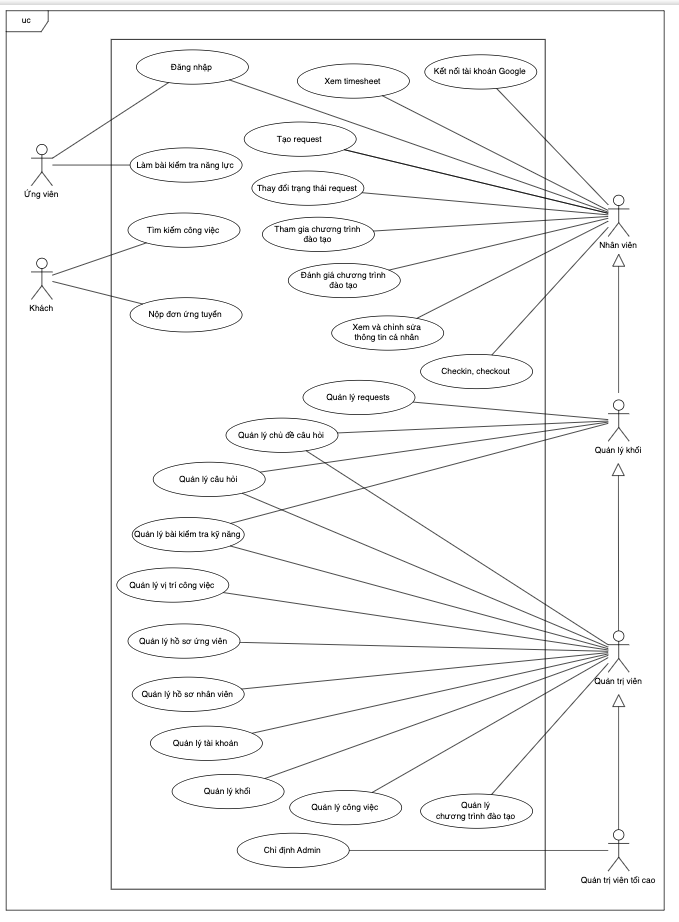
\includegraphics[width=\linewidth]{Hinhve/UC_TongQuan.png}
    \caption{Biểu đồ usecase tổng quan}
\end{figure}

Hệ thống bao gồm sáu tác nhân là Khách (Guest), Ứng viên (Candidate), Nhân viên (Employee) , Quản lý khối (Division Manager), Quản trị viên (Admin) và Quản trị viên tối cao (Super Admin)

\noindent Tác nhân \textbf{Khách} có các chức năng:
\begin{itemize}
\item Tìm kiếm việc làm: Tìm kiếm các công việc đang cần tuyển, lọc công việc theo một số tiêu chí
\item Xem thông tin chi tiết của công việc
\item Nộp đơn ứng tuyển: Điền thông tin cá nhân, vị trí muốn ứng tuyển và gửi đơn ứng tuyển về hệ thống
\end{itemize}

\noindent Tác nhân \textbf{Ứng viên} có các chức năng:
\begin{itemize}
\item Đăng nhập: Đăng nhập vào hệ thống sử dụng tài khoản (email và password) do bộ phận nhân sự cấp hoặc đăng nhập bằng Google
\item Xem danh sách bài kiểm tra được chỉ định
\item Làm bài kiểm tra năng lực do bộ phận nhân sự của công ty đã chỉ định và nhận kết quả sơ bộ của bài kiểm tra đó
\item Nhận các thông báo qua email đã đăng ký
\item Đăng xuất: Đăng xuất khỏi hệ thống
\end{itemize}

\noindent Tác nhân \textbf{Nhân viên} có các chức năng:
\begin{itemize}
\item Đăng nhập: Đăng nhập vào hệ thống bằng tài khoản (email và password) được cấp hoặc đăng nhập bằng Google
\item Xem và thay đổi một số thông tin cá nhân, mật khẩu tài khoản
\item Check in, check out
\item Tạo đơn: Tạo các đơn (request) để xin nghỉ làm, xin làm từ xa, làm tăng ca (Overtime), xin check in, check out bù
\item Xem lịch làm việc của bản thân (Timesheet)
\item Xem, tham gia và đánh giá các chương trình đào tạo
\item Liên kết tài khoản Google để có thể đăng nhập bằng tài khoản Google
\item Đăng xuất: Đăng xuất khỏi hệ thống
\end{itemize}

\noindent Tác nhân \textbf{Quản lý khối} có các chức năng của nhân viên và có thêm các tính năng:
\begin{itemize}
\item Quản lý đơn của nhân viên trong khối của mình quản lý
\item Thêm câu hỏi, tạo các bài kiểm tra
\end{itemize}

\noindent Tác nhân \textbf{Quản trị viên} có các chức năng của nhân viên và có thêm các tính năng:
\begin{itemize}
\item Quản lý đơn của tất các nhân viên
\item Quản lý các khối trong công ty
\item Quản lý các vị trí công việc của công ty
\item Quản lý hồ sơ ứng viên
\item Quản lý hồ sơ nhân viên
\item Quản lý tài khoản trong hệ thống
\item Quản lý các chương trình đào tạo
\item Quản lý các công việc cần tuyển nhân sự
\item Chỉ định bài kiểm tra cho ứng viên
\item Xem các báo cáo thống kê
\end{itemize}

\noindent Tác nhân \textbf{Quản trị viên tối cao} có các chức năng của Quản trị viên và có thêm các tính năng:
\begin{itemize}
\item Chỉ định nhân viên lên làm Quản trị viên
\end{itemize}

\subsection{Biểu đồ use case phân rã "Đăng nhập"}
\label{subsection:2.2.2}
\begin{figure}[h]
    \centering
    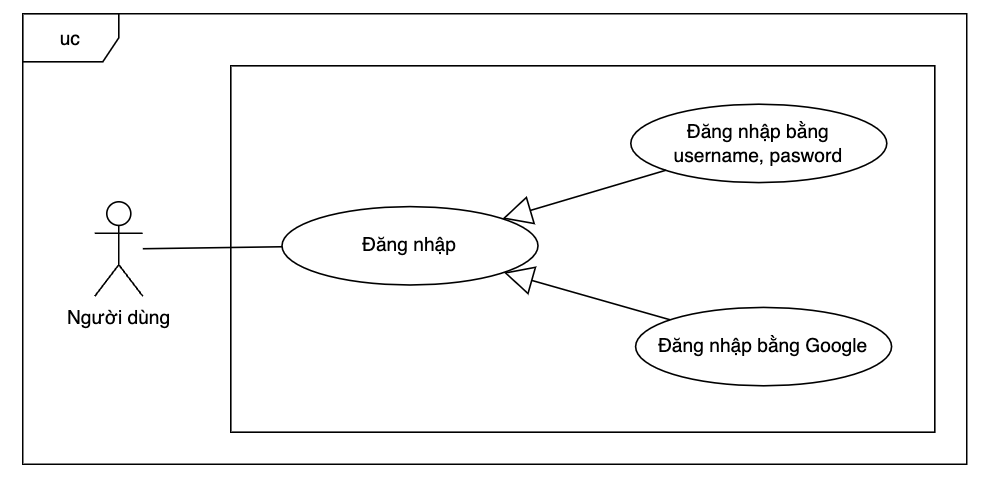
\includegraphics[width=0.9\textwidth]{Hinhve/UC_DangNhap.png}
    \caption{Biểu đồ usecase phân rã "Đăng nhập"}
\end{figure}
Use case này cho phép những người dùng có tài khoản trên hệ thống đăng nhập và sử dụng các tài nguyên của hệ thống theo quyền hạn của mình.

\subsection{Biểu đồ use case phân rã "Quản lý hồ sơ ứng viên"}
\label{subsection:2.2.3}
\begin{figure}[H]
    \centering
    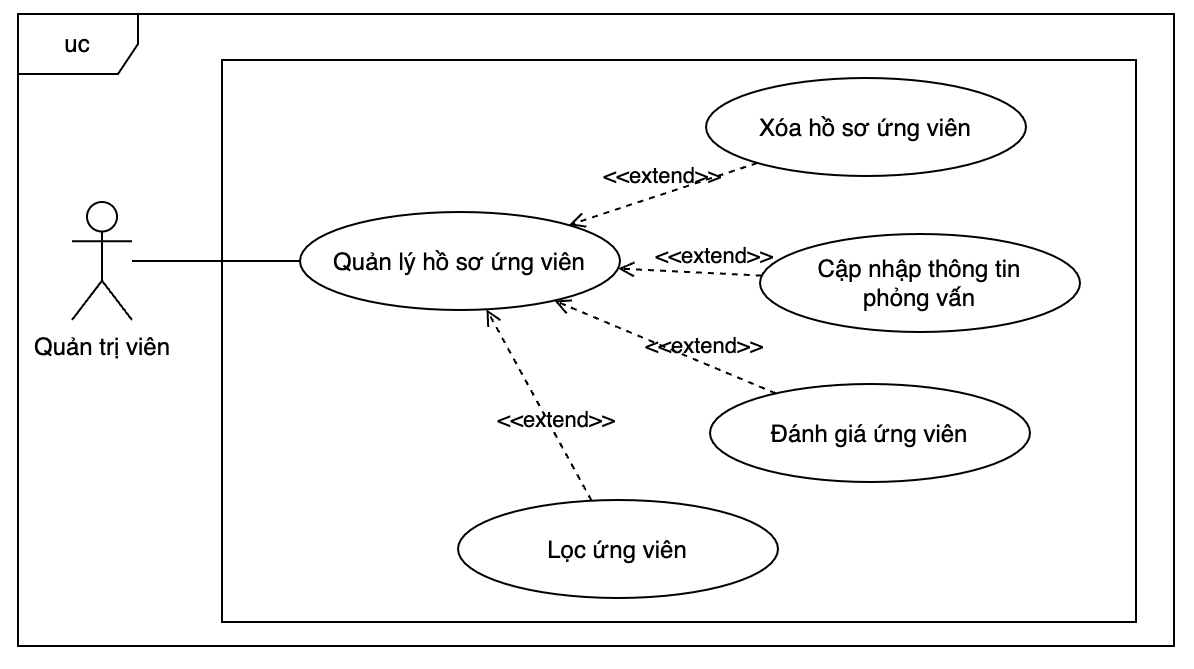
\includegraphics[width=0.9\textwidth]{Hinhve/UC_QuanLyHoSoUngVien.png}
    \caption{Biểu đồ usecase phân rã "Quản lý hồ sơ ứng viên"}
\end{figure}
Use case này cho phép quản trị viên của hệ thống quản lý hồ sơ cá nhân của các ứng viên.

\subsection{Biểu đồ use case phân rã "Quản lý hồ sơ nhân viên"}
\label{subsection:2.2.4}
\begin{figure}[H]
    \centering
    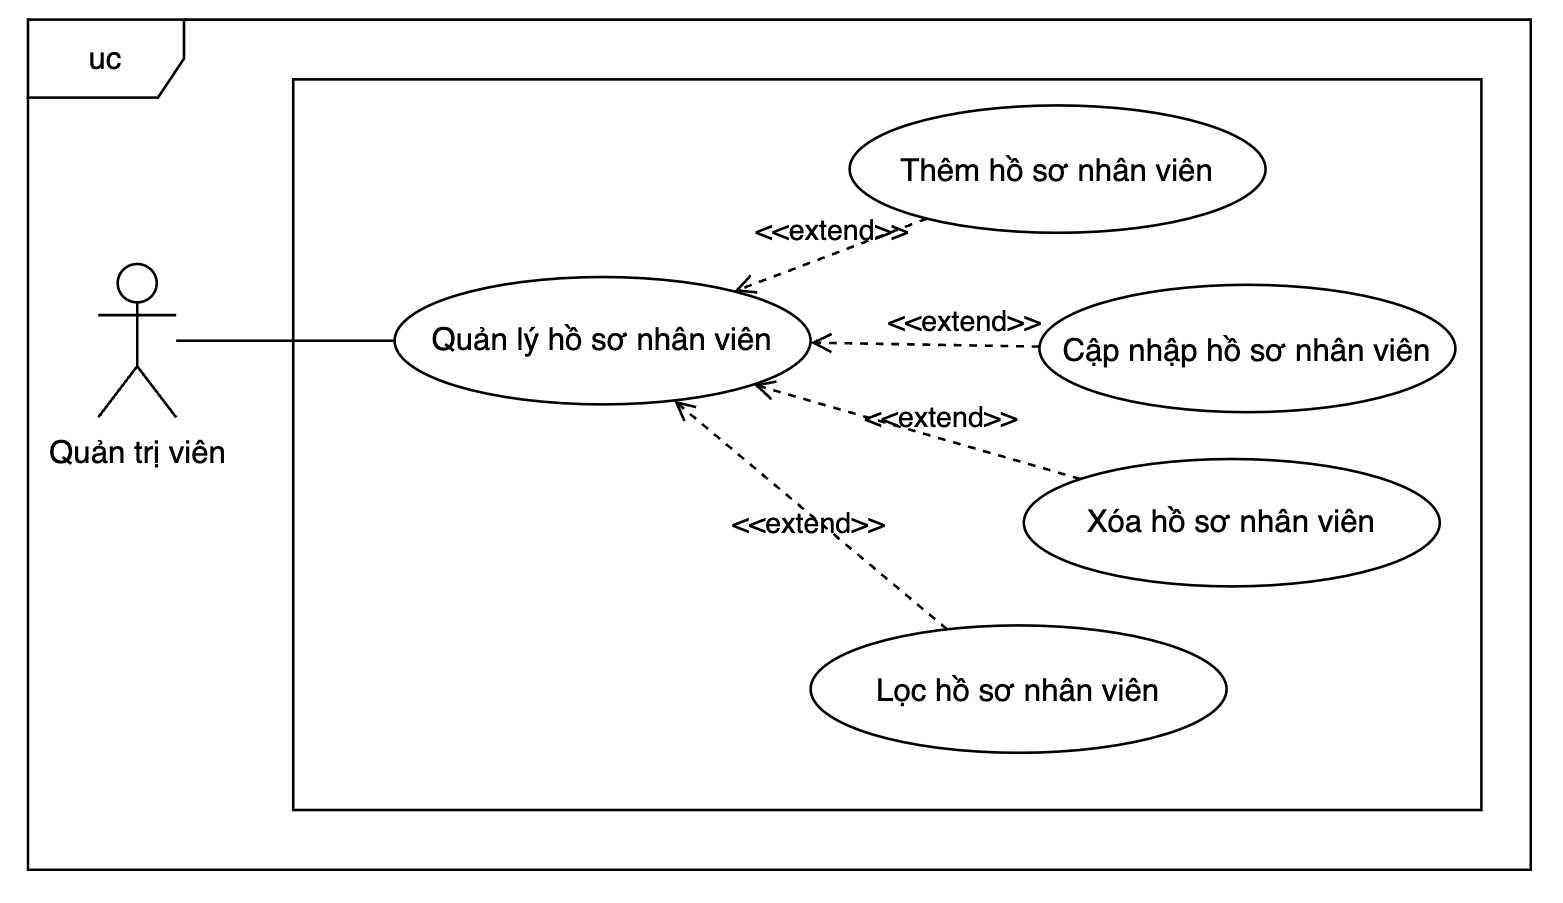
\includegraphics[width=0.9\textwidth]{Hinhve/UC_QuanLyHoSoNhanVien.png}
    \caption{Biểu đồ usecase phân rã "Quản lý hồ sơ nhân viên"}
\end{figure}
Use case này cho phép quản trị viên của hệ thống quản lý hồ sơ cá nhân của các nhân viên trong công ty.

\subsection{Biểu đồ use case phân rã "Quản lý khối"}
\label{subsection:2.2.5}
\begin{figure}[H]
    \centering
    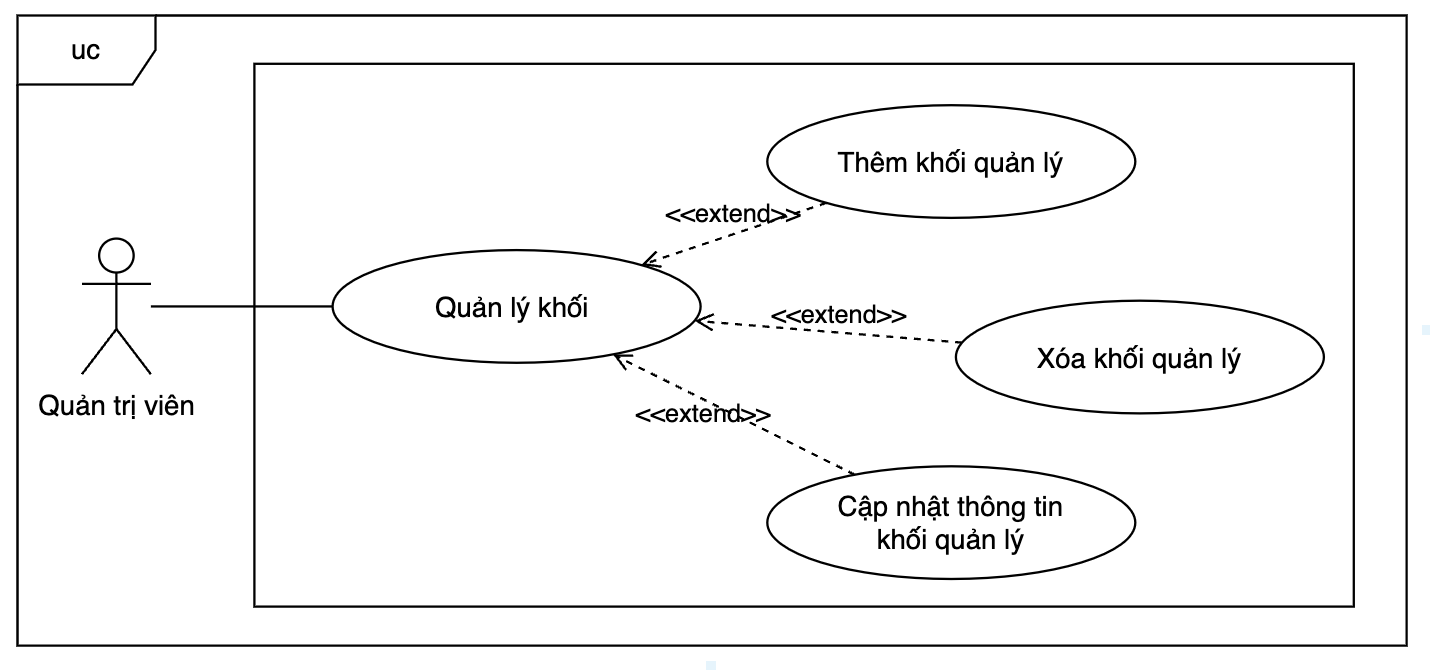
\includegraphics[width=0.9\textwidth]{Hinhve/UC_QuanLyKhoi.png}
    \caption{Biểu đồ usecase phân rã "Quản lý khối"}
\end{figure}
Đối với một công ty có quy mô trung bình trở lên việc chia thành các khối, ban ngành để quản lý sẽ hiệu quả hơn. Vì thế use case này giúp các quản trị viên quản lý được các khối ngành trong công ty.

\subsection{Biểu đồ use case phân rã "Quản lý vị trí công việc"}
\label{subsection:2.2.6}
\begin{figure}[H]
    \centering
    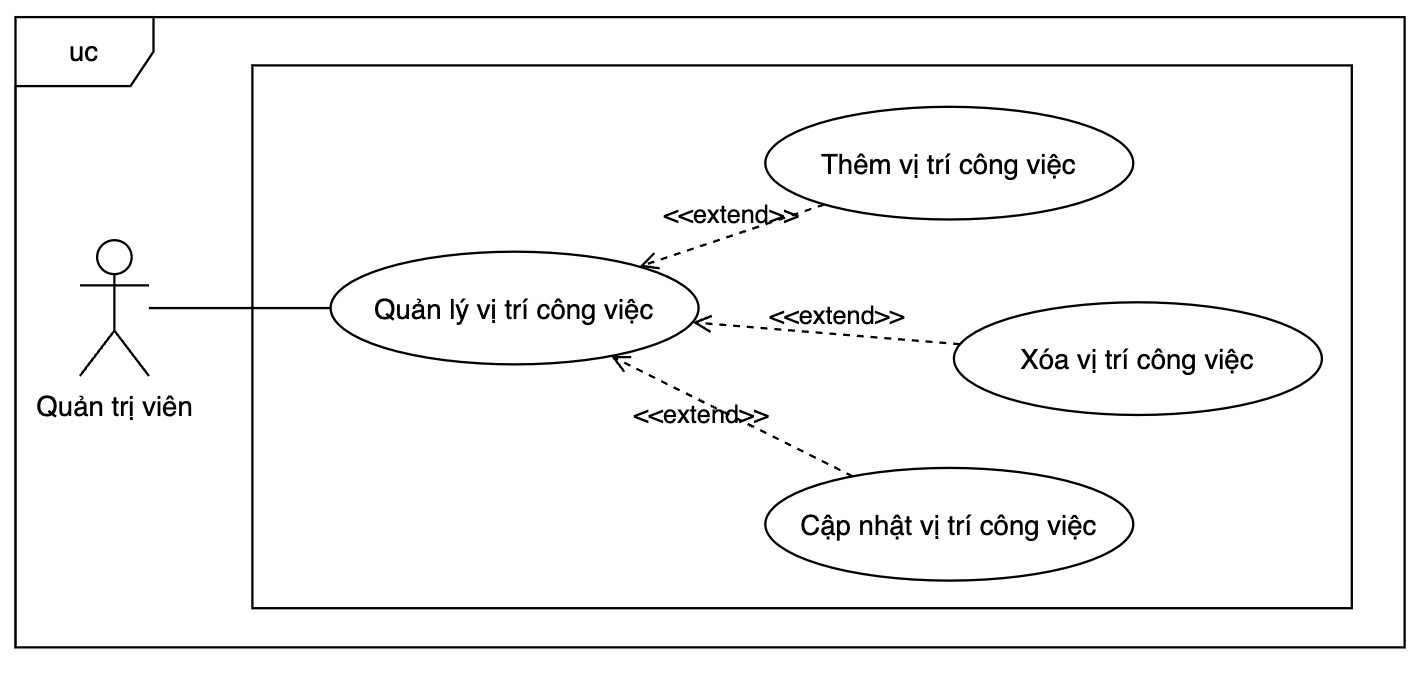
\includegraphics[width=0.9\textwidth]{Hinhve/UC_QuanLyViTriCongViec.png}
    \caption{Biểu đồ usecase phân rã "Quản lý vị trí công việc"}
\end{figure}
Mỗi công ty lại có những vị trí công việc khác nhau chẳng hạn như kế toán, lập trình viên frontend, nhân viên sale,... Use case này giúp các quản trị viên quản lý được các vị trí công việc như vậy.

\subsection{Biểu đồ use case phân rã "Quản lý tài khoản"}
\label{subsection:2.2.7}
\begin{figure}[H]
    \centering
    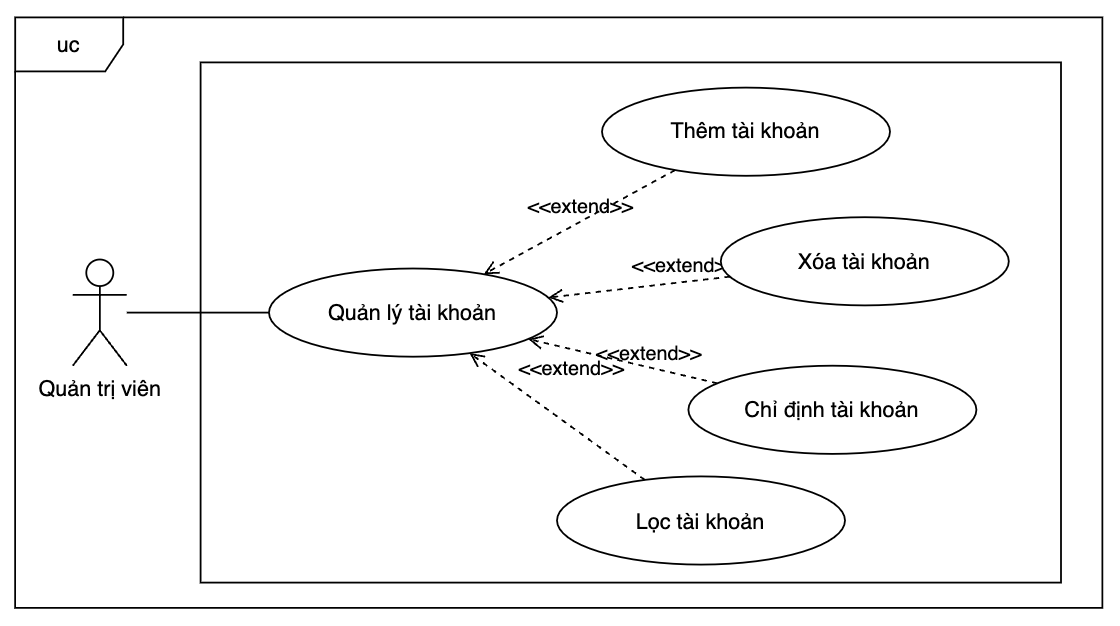
\includegraphics[width=0.9\textwidth]{Hinhve/UC_QuanLyTaiKhoan.png}
    \caption{Biểu đồ usecase phân rã "Quản lý tài khoản"}
\end{figure}
Use case này hỗ trợ các quản trị viên quản lý các tài khoản để đăng nhập vào hệ thống.

\subsection{Biểu đồ use case phân rã "Quản lý request"}
\label{subsection:2.2.8}
\begin{figure}[H]
    \centering
    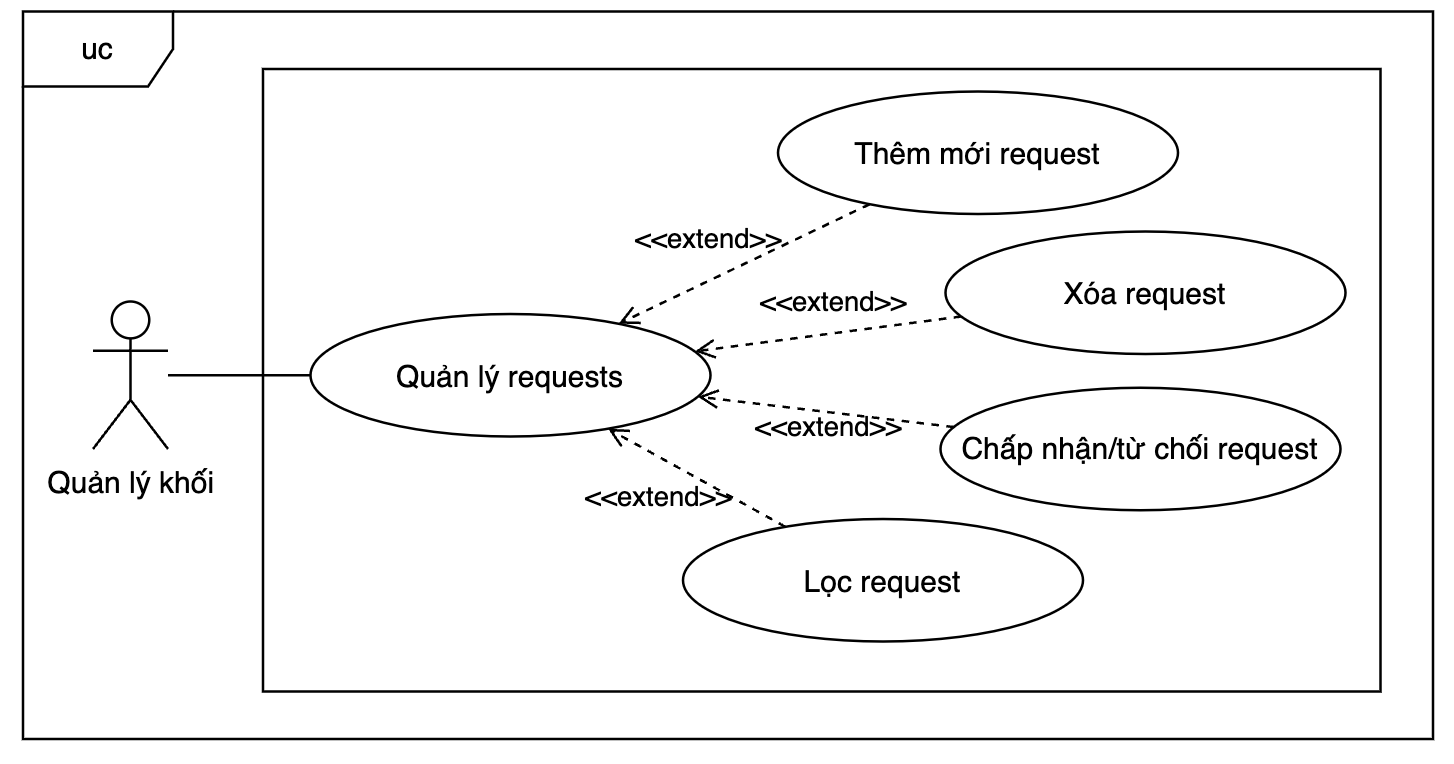
\includegraphics[width=0.9\textwidth]{Hinhve/UC_QuanLyRequest.png}
    \caption{Biểu đồ usecase phân rã "Quản lý request"}
\end{figure}
Với use case này, các nhân viên của công ty có thể tạo các request chẳng hạn xin nghỉ, xin làm từ xa,... và bộ phận nhân sự sẽ phê duyệt các request này.

\subsection{Biểu đồ use case phân rã "Quản lý câu hỏi"}
\label{subsection:2.2.9}
\begin{figure}[H]
    \centering
    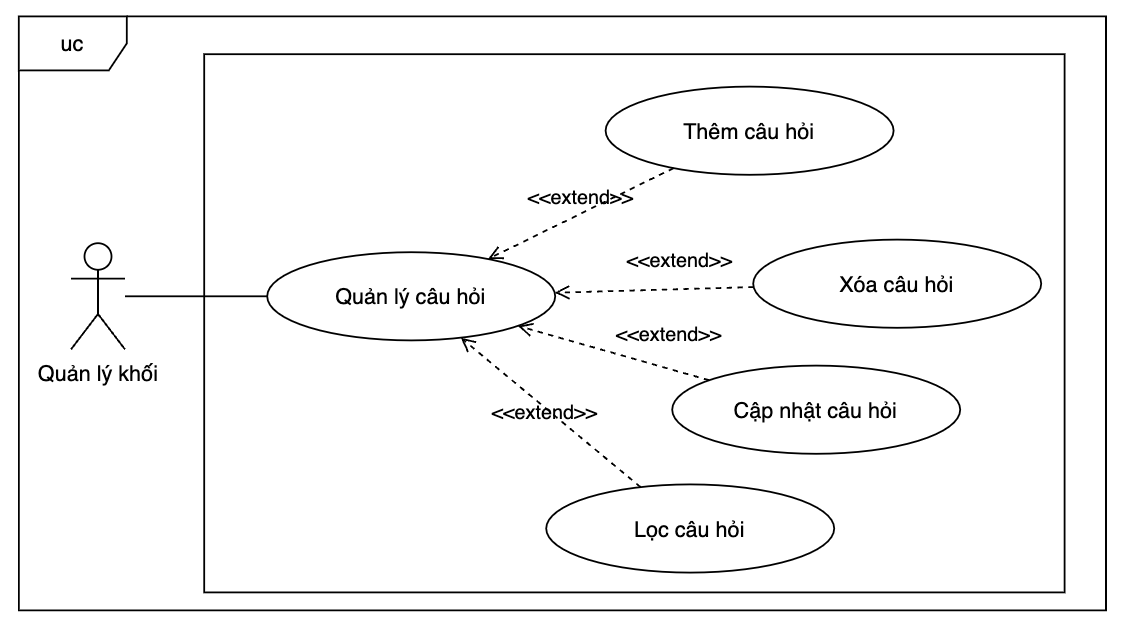
\includegraphics[width=0.9\textwidth]{Hinhve/UC_QuanLyCauHoi.png}
    \caption{Biểu đồ usecase phân rã "Quản lý câu hỏi"}
\end{figure}
Để tạo các bài kiểm tra kỹ năng thì cần có các câu hỏi, vì thế use case này giúp quản lý việc thêm, sửa hay xóa các câu hỏi.

\subsection{Biểu đồ use case phân rã "Quản lý chủ đề câu hỏi"}
\label{subsection:2.2.10}
\begin{figure}[H]
    \centering
    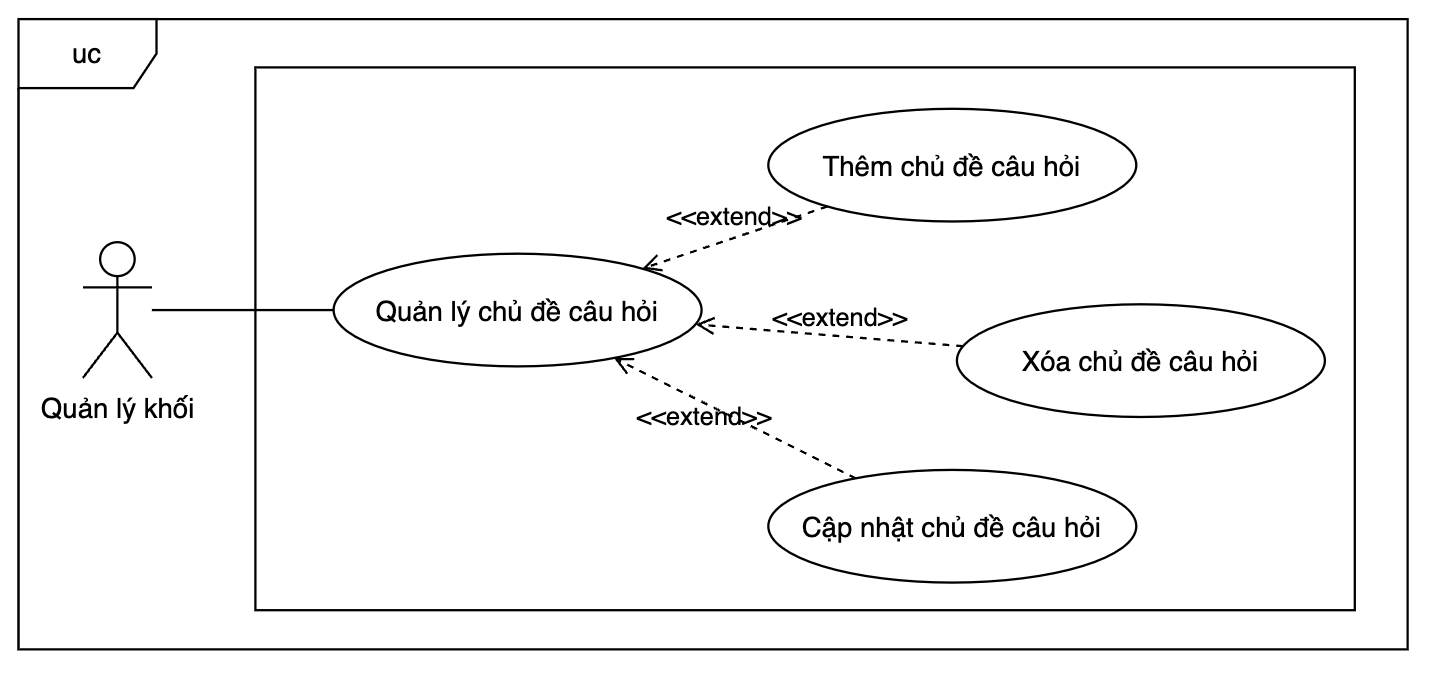
\includegraphics[width=0.9\textwidth]{Hinhve/UC_QuanLyChuDeCauHoi.png}
    \caption{Biểu đồ usecase phân rã "Quản lý chủ đề câu hỏi"}
\end{figure}
Mỗi câu hỏi sẽ thuộc vào một chủ đề nào đó. Use case này sẽ giúp quản lý các chủ đề câu hỏi đó.

\subsection{Biểu đồ use case phân rã "Quản lý bài kiểm tra kỹ năng"}
\label{subsection:2.2.11}
\begin{figure}[H]
    \centering
    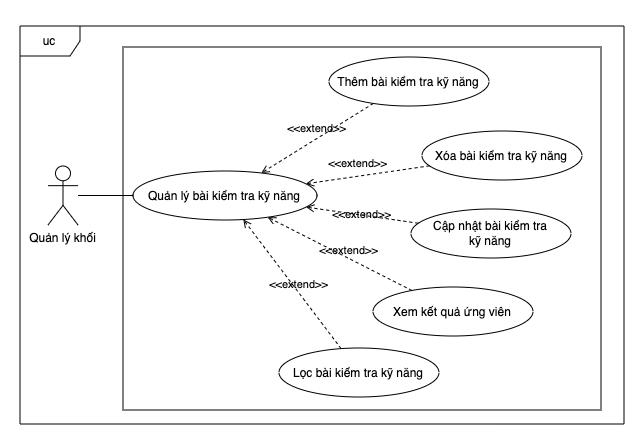
\includegraphics[width=0.9\textwidth]{Hinhve/UC_QuanLyBaiKiemTraKyNang.png}
    \caption{Biểu đồ usecase phân rã "Quản lý bài kiểm tra kỹ năng"}
\end{figure}
Use case này cho phép quản lý các bài kiểm tra kỹ năng, quản trị viên cũng có thể xem được kết quả làm bài của các thí sinh.

\subsection{Biểu đồ use case phân rã "Quản lý công việc"}
\label{subsection:2.2.12}
\begin{figure}[H]
    \centering
    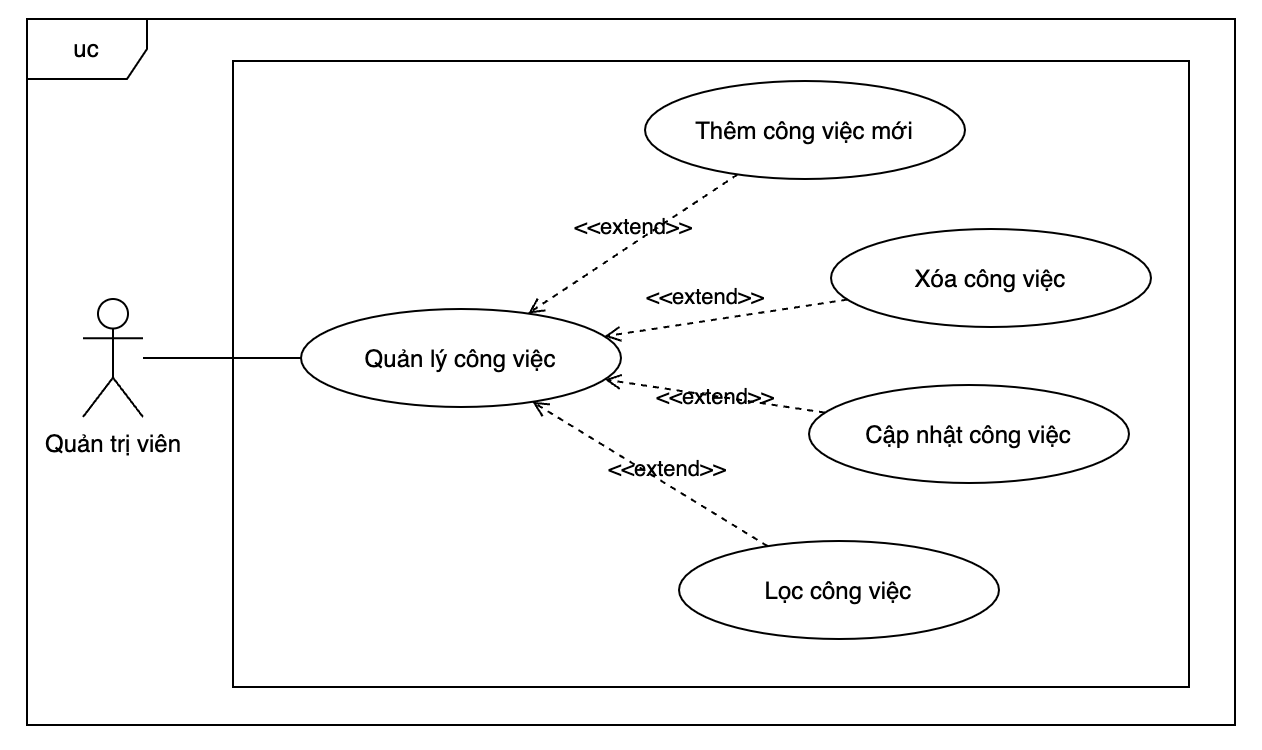
\includegraphics[width=0.9\textwidth]{Hinhve/UC_QuanLyCongViec.png}
    \caption{Biểu đồ usecase phân rã "Quản lý công việc"}
\end{figure}
Ở mỗi vị trí công việc thì lại có nhiều đầu việc khác nhau, chẳng hạn như cùng là vị trí lập trình viên frontend có thể sinh ra các đầu việc như lập trình viên ReactJS, lập trình viên VueJS,... Use case này giúp quản lý các loại công việc như vậy.

\subsection{Biểu đồ use case phân rã "Quản lý chương trình đào tạo"}
\label{subsection:2.2.13}
\begin{figure}[H]
    \centering
    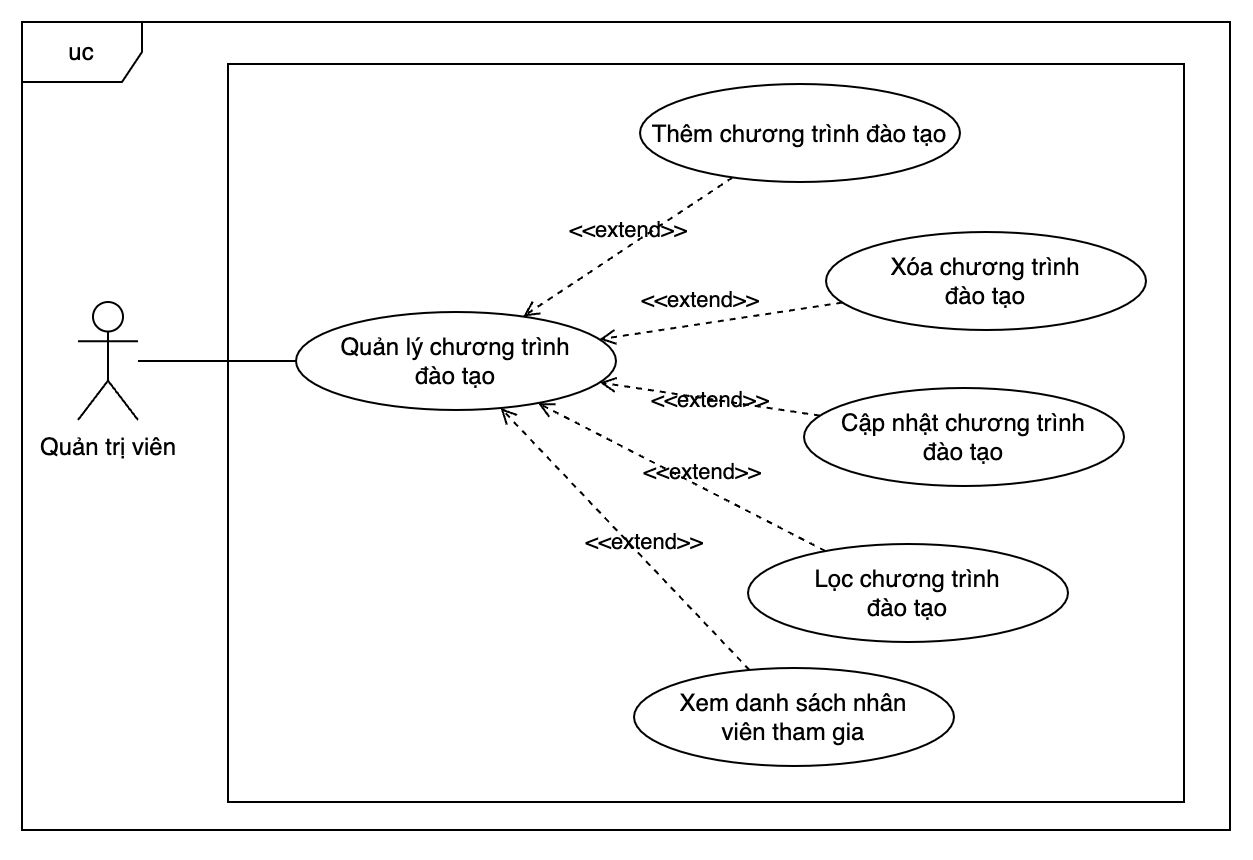
\includegraphics[width=0.9\textwidth]{Hinhve/UC_QuanLyChuongTrinhDaoTao.png}
    \caption{Biểu đồ usecase phân rã "Quản lý chương trình đào tạo"}
\end{figure}
Để có nguồn nhân lực chất lượng hơn thì mỗi công ty thường có các chương trình đào tạo. Vì vậy use case này giúp quản trị viên quản lý các chương trình đào tạo đó.

\subsection{Quy trình nghiệp vụ}
\label{subsection:2.2.14}
\textbf{Biểu đồ hoạt động: Làm bài kiểm tra kỹ năng:}

Ở luồng hoạt động này, quản trị viên cần phải tạo tài khoản và chỉ định bài kiểm tra kỹ năng cho ứng viên. Ứng viên dùng tài khoản đó đăng nhập vào hệ thống và làm bài kiểm tra đã được chỉ định. Trong quá trình làm bài, nếu ứng viên nộp bài kiểm tra đúng thời hạn thì kết quả bài kiểm tra sẽ được ghi nhận. Ngược lại, kết quả bài kiểm tra sẽ không được công nhận và bài kiểm tra được đánh dấu là hoàn thành (Đồng nghĩa với việc ứng viên không thể làm lại lần hai)
\begin{figure}[H]
    \centering
    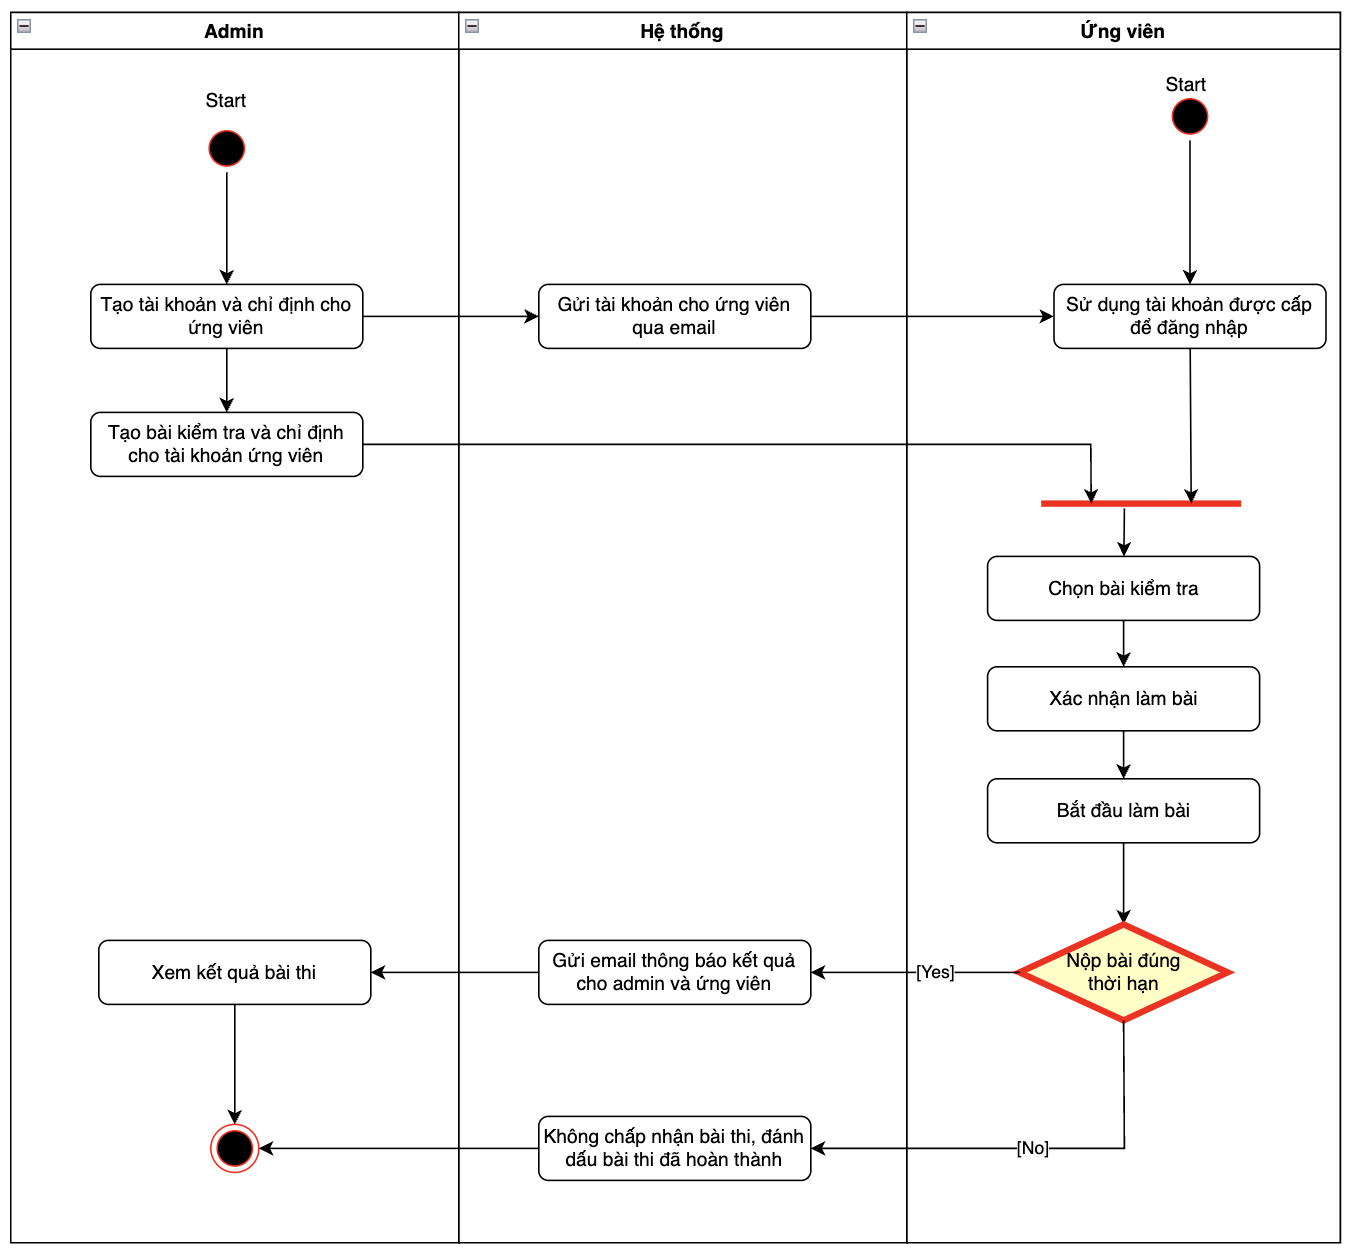
\includegraphics[width=0.9\textwidth]{Hinhve/AD_LamBaiKiemTraKyNang.png}
    \caption{Biểu đồ hoạt động "Làm bài kiểm tra kỹ năng"}
\end{figure}

\textbf{Biểu đồ hoạt động: Hủy bỏ request:}

Khi nhân viên tạo một request, nhân viên có thể hủy được request này trong một số trường hợp. Nếu request đó chưa từng bị hủy, cũng chưa được duyệt thì khi nhân viên yêu cầu hủy request hệ thống sẽ xóa request này khỏi hệ thống. Trường hợp request chưa từng bị hủy và đã từng được duyệt, nếu nhân viên yêu cầu hủy request và người duyệt request chấp nhận thì hệ thống sẽ xóa request. Trường hợp request đã từng bị hủy trước đó, hệ thống sẽ không hiển thị nút hủy do đó nhân viên không thể hủy request.
\begin{figure}[H]
    \centering
    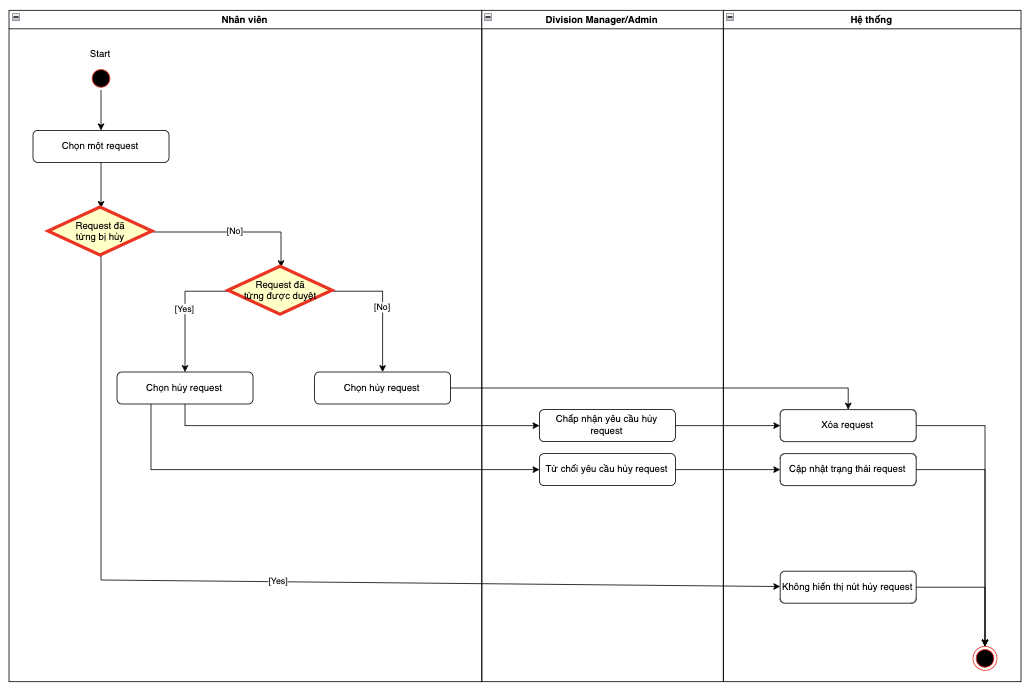
\includegraphics[width=0.9\textwidth]{Hinhve/AD_HuyRequest.png}
    \caption{Biểu đồ hoạt động "Hủy bỏ request"}
\end{figure}

\textbf{Biểu đồ hoạt động: Tham gia và đánh giá chương trình đào tạo:}

Để tham gia chương trình đào tạo, chương trình đó phải chưa diễn ra. Trong trường hợp chương trình đã diễn ra rồi và nhân viên có tham gia chương trình đó thì hệ thống sẽ hiển thị module đánh giá và nhân viên có thể đánh giá chương trình đào tạo. Sau khi nhân viên đánh giá thành công, hệ thống sẽ tính toán lại số điểm trung bình của chương trình đào tạo.
\begin{figure}[H]
    \centering
    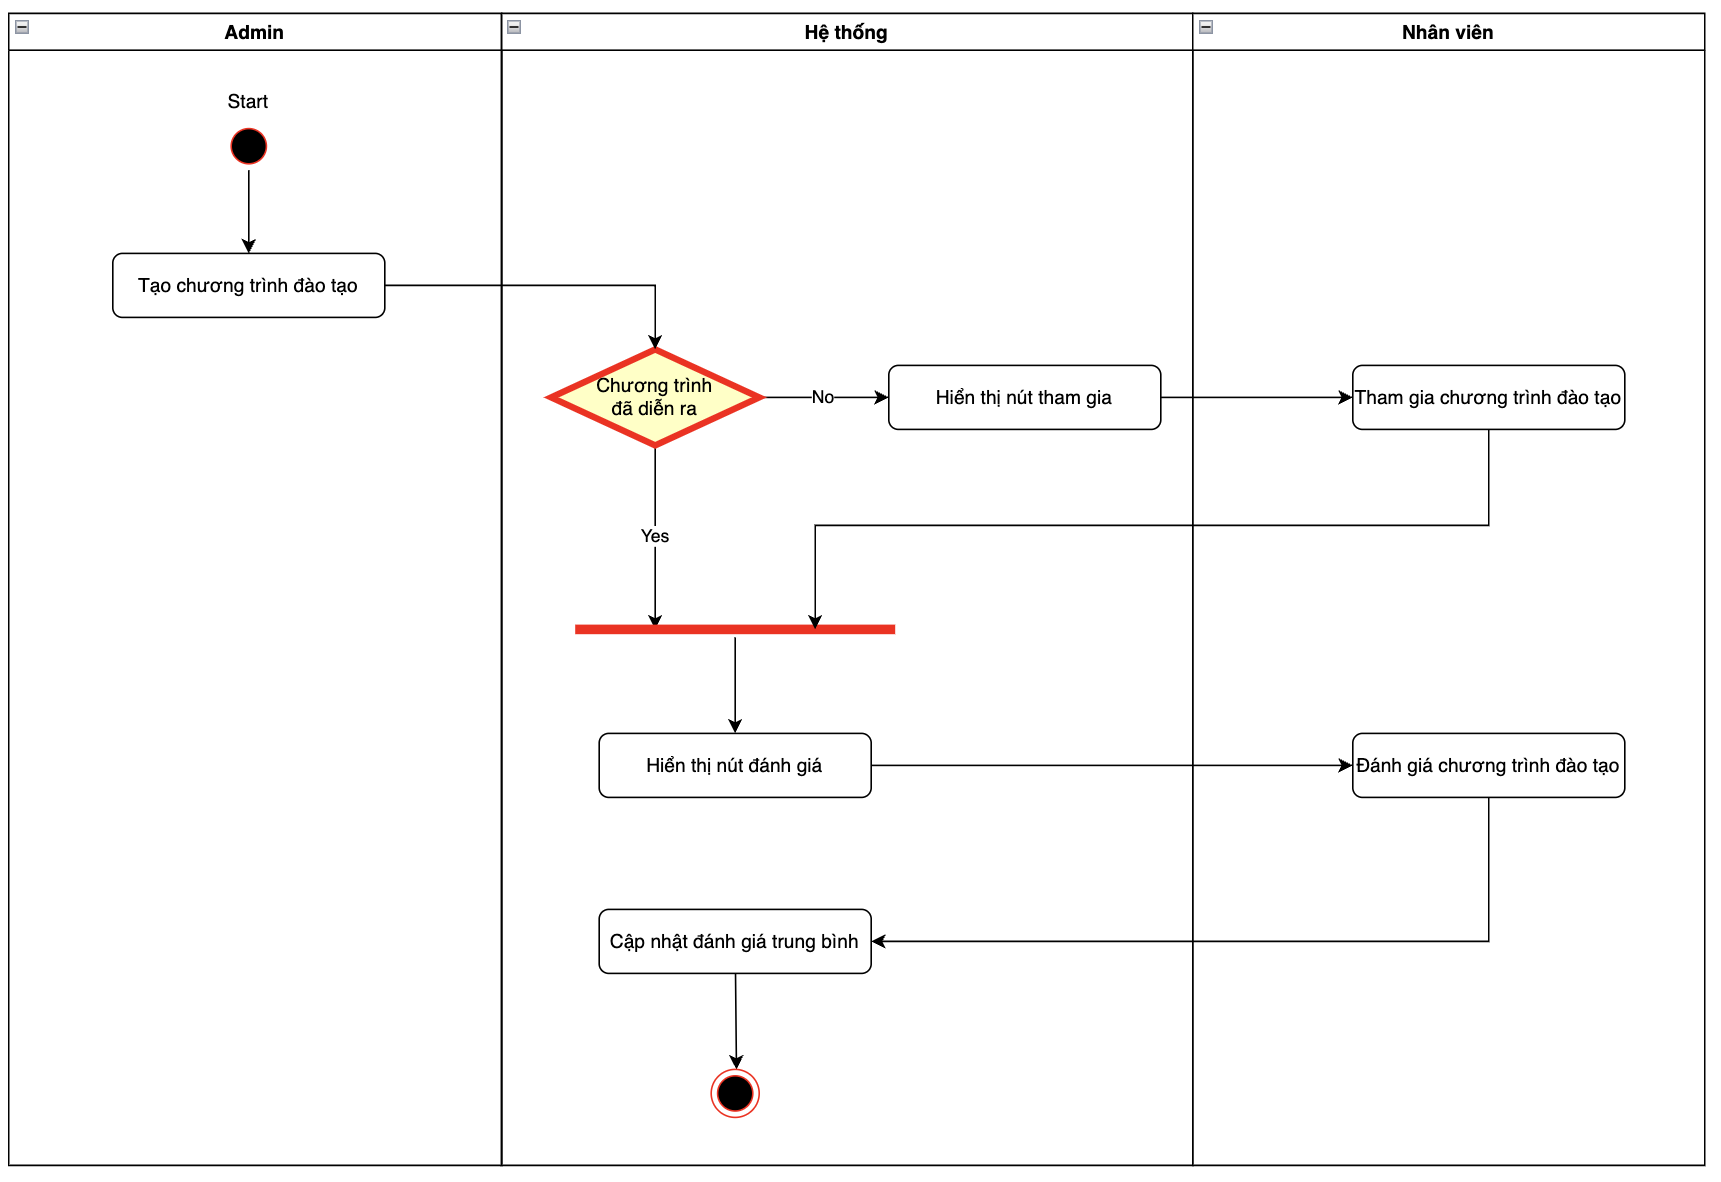
\includegraphics[width=0.9\textwidth]{Hinhve/AD_ThamGiaDanhGiaChuongTrinhDaoTao.png}
    \caption{Biểu đồ hoạt động "Tham gia và đánh giá chương trình đào tạo"}
\end{figure}

\section{Đặc tả chức năng}
\label{section:2.3}
\subsection{Đặc tả use case "Tìm kiếm việc làm"}
\begin{longtable}{|p{0.15\textwidth}|p{0.1\textwidth}p{0.23\textwidth}p{0.4\textwidth}|}
\caption{Bảng đặc tả usecase "Tìm kiếm việc làm"}
\hline
\textbf{Mã usecase} & \multicolumn{1}{p{0.1\textwidth}|}{UC01} & \multicolumn{1}{p{0.23\textwidth}|}{\textbf{Tên usecase}} & Tìm kiếm việc làm \\ \hline
\textbf{Tác nhân} & \multicolumn{3}{p{0.73\textwidth}|}{Khách} \\ \hline
\textbf{Mô tả} & \multicolumn{3}{p{0.73\textwidth}|}{Cho phép khách tìm kiếm việc làm trên hệ thống} \\ \hline
\textbf{Tiền điều kiện} & \multicolumn{3}{p{0.73\textwidth}|}{Không} \\ \hline
& \multicolumn{1}{l|}{\textbf{STT}} & \multicolumn{1}{l|}{\textbf{Thực hiện bởi}} & \textbf{Hành động} \\ \cline{2-4} 
& \multicolumn{1}{l|}{1} & \multicolumn{1}{l|}{Khách} & Chọn chức năng Tìm kiếm việc làm \\ \cline{2-4} 
& \multicolumn{1}{l|}{2} & \multicolumn{1}{l|}{Hệ thống} & Hiển thị giao diện tìm kiếm \\ \cline{2-4}
\multirow{-4}{\multicolumn{1}{p{0.15\textwidth}|}{\textbf{Luồng sự kiện chính}}}
& \multicolumn{1}{l|}{3} & \multicolumn{1}{l|}{Khách} & Nhập từ khóa hoặc lựa chọn hình thức làm việc, vị trí công việc,... \\ \cline{2-4}
\hline
& \multicolumn{1}{l|}{4} & \multicolumn{1}{l|}{Hệ thống} & Truy vấn theo dữ liệu tìm kiếm \\ \cline{2-4} 
& \multicolumn{1}{l|}{5} & \multicolumn{1}{l|}{Hệ thống} & Hiển thị danh sách việc làm tương ứng với các từ khóa tìm kiếm \\ \hline
& \multicolumn{1}{l|}{\textbf{STT}} & \multicolumn{1}{l|}{\textbf{Thực hiện bởi}} & \textbf{Hành động} \\ \cline{2-4} 
\multirow{-2}{\multicolumn{1}{p{0.15\textwidth}|}{\textbf{Luồng sự kiện thay thế}}}    
& \multicolumn{1}{l|}{5a} & \multicolumn{1}{l|}{Hệ thống} & Nếu không tìm thấy kết quả phù hợp với dữ liệu tìm kiếm thì hiển thị thông báo không có kết quả phù hợp \\ \hline
\textbf{Hậu điều kiện} & \multicolumn{3}{p{0.73\textwidth}|}{Không} \\ \hline
\end{longtable}

\subsection{Đặc tả use case "Nộp đơn ứng tuyển"}
\begin{longtable}{|p{0.15\textwidth}|p{0.1\textwidth}p{0.23\textwidth}p{0.4\textwidth}|}
\caption{Bảng đặc tả usecase "Nộp đơn ứng tuyển"}
\hline
\textbf{Mã usecase} & \multicolumn{1}{p{0.1\textwidth}|}{UC02} & \multicolumn{1}{p{0.23\textwidth}|}{\textbf{Tên usecase}} & Nộp đơn ứng tuyển \\ \hline
\textbf{Tác nhân} & \multicolumn{3}{p{0.73\textwidth}|}{Khách} \\ \hline
\textbf{Mô tả} & \multicolumn{3}{p{0.73\textwidth}|}{Cho phép khách gửi đơn ứng tuyển về hệ thống} \\ \hline
\textbf{Tiền điều kiện} & \multicolumn{3}{p{0.73\textwidth}|}{Không} \\ \hline
& \multicolumn{1}{l|}{\textbf{STT}} & \multicolumn{1}{l|}{\textbf{Thực hiện bởi}} & \textbf{Hành động} \\ \cline{2-4} 
\hline
& \multicolumn{1}{l|}{1} & \multicolumn{1}{l|}{Khách} & Chọn chức năng nộp đơn ứng tuyển \\ \cline{2-4} 
& \multicolumn{1}{l|}{2} & \multicolumn{1}{l|}{Hệ thống} & Hiển thị giao diện form điền thông tin \\ \cline{2-4}
\multirow{-3}{\multicolumn{1}{p{0.15\textwidth}|}{\textbf{Luồng sự kiện chính}}}
& \multicolumn{1}{l|}{3} & \multicolumn{1}{l|}{Khách} & Nhập các thông tin cơ bản (Tên, email, số điện thoại, công việc muốn ứng tuyển, file CV) và bấm nút gửi đơn \\ \cline{2-4} \hline
& \multicolumn{1}{l|}{4} & \multicolumn{1}{l|}{Hệ thống} & Kiểm tra dữ liệu khách vừa nhập \\ \cline{2-4} 
& \multicolumn{1}{l|}{5} & \multicolumn{1}{l|}{Hệ thống} & Tạo một hồ sơ mới \\ \cline{2-4}
& \multicolumn{1}{l|}{6} & \multicolumn{1}{l|}{Hệ thống} & Thông tin hợp lệ, tạo một đơn ứng tuyển mới và hiển thị thông báo đã nộp đơn thành công \\ \hline
& \multicolumn{1}{l|}{\textbf{STT}} & \multicolumn{1}{l|}{\textbf{Thực hiện bởi}} & \textbf{Hành động} \\ \cline{2-4} 
\multirow{-3}{\multicolumn{1}{p{0.15\textwidth}|}{\textbf{Luồng sự kiện thay thế}}}    
& \multicolumn{1}{l|}{5a} & \multicolumn{1}{l|}{Hệ thống} & Thông tin khách nhập chưa hợp lệ, yêu cầu sửa lại \\ \hline
\textbf{Hậu điều kiện} & \multicolumn{3}{p{0.73\textwidth}|}{Hệ thống lưu đơn ứng tuyển vào cơ sở dữ liệu} \\ \hline
\end{longtable}

\subsection{Đặc tả use case "Làm bài kiểm tra năng lực"}
\begin{longtable}{|p{0.15\textwidth}|p{0.1\textwidth}p{0.23\textwidth}p{0.4\textwidth}|}
\caption{Bảng đặc tả usecase "Làm bài kiểm tra năng lực"}
\hline
\textbf{Mã usecase} & \multicolumn{1}{p{0.1\textwidth}|}{UC03} & \multicolumn{1}{p{0.23\textwidth}|}{\textbf{Tên usecase}} & Làm bài kiểm tra năng lực \\ \hline
\textbf{Tác nhân} & \multicolumn{3}{p{0.73\textwidth}|}{Ứng viên} \\ \hline
\textbf{Mô tả} & \multicolumn{3}{p{0.73\textwidth}|}{Ứng viên làm bài kiểm tra năng lực do bộ phận nhân sự chỉ định} \\ \hline
\textbf{Tiền điều kiện} & \multicolumn{3}{p{0.73\textwidth}|}{Ứng viên đã đăng nhập vào hệ thống} \\ \hline
& \multicolumn{1}{l|}{\textbf{STT}} & \multicolumn{1}{l|}{\textbf{Thực hiện bởi}} & \textbf{Hành động} \\ \cline{2-4} 
& \multicolumn{1}{l|}{1} & \multicolumn{1}{l|}{Ứng viên} & Chọn bài kiểm tra năng lực được chỉ định \\ \cline{2-4} 
& \multicolumn{1}{l|}{2} & \multicolumn{1}{l|}{Hệ thống} & Hiển thị chú ý bài kiểm tra chỉ được thực hiện một lần và nút xác nhận làm bài \\ \cline{2-4} 
& \multicolumn{1}{l|}{3} & \multicolumn{1}{l|}{Ứng viên} & Nhấn nút xác nhận làm bài \\ \cline{2-4} 
& \multicolumn{1}{l|}{4} & \multicolumn{1}{l|}{Hệ thống} & Hiển thị bài kiểm tra và bắt đầu đếm ngược thời gian làm bài \\ \cline{2-4} \hline
\multirow{-2}{\multicolumn{1}{p{0.15\textwidth}|}{\textbf{Luồng sự kiện chính}}}       
& \multicolumn{1}{l|}{5} & \multicolumn{1}{l|}{Ứng viên} & Nộp bài trước thời gian kết thúc \\ \cline{2-4}
& \multicolumn{1}{l|}{6} & \multicolumn{1}{l|}{Hệ thống} & Ghi nhận kết quả làm bài, tính toán kết quả sơ bộ và hiển thị kết quả sơ bộ \\ \cline{2-4}
& \multicolumn{1}{l|}{7} & \multicolumn{1}{l|}{Hệ thống} & Gửi một email thông báo nộp bài thành công và một số thông tin cần thiết khác về quy trình tuyển dụng \\ \hline
& \multicolumn{1}{l|}{\textbf{STT}} & \multicolumn{1}{l|}{\textbf{Thực hiện bởi}} & \textbf{Hành động} \\ \cline{2-4}   
& \multicolumn{1}{l|}{5a} & \multicolumn{1}{l|}{Ứng viên} & Thời gian đã hết và ứng viên chưa nộp bài \\ \cline{2-4}   
\multirow{-4}{\multicolumn{1}{p{0.15\textwidth}|}{\textbf{Luồng sự kiện thay thế}}}  
& \multicolumn{1}{l|}{6a} & \multicolumn{1}{l|}{Hệ thống} & Hệ thống tự động nộp bài dựa trên những câu trả lời của ứng viên \\ \cline{2-4}  
& \multicolumn{1}{l|}{5b} & \multicolumn{1}{l|}{Ứng viên} & Thời gian đã hết và ứng viên thoát ra \\ \cline{2-4}   
& \multicolumn{1}{l|}{6b} & \multicolumn{1}{l|}{Hệ thống} & Hệ thống không ghi nhận kết quả bài kiểm tra \\ \hline
\textbf{Hậu điều kiện} & \multicolumn{3}{p{0.73\textwidth}|}{Hệ thống lưu kết quả bài kiểm tra vào cơ sở dữ liệu} \\ \hline
\end{longtable}

\subsection{Đặc tả use case "Tạo request"}
\begin{longtable}{|p{0.15\textwidth}|p{0.1\textwidth}p{0.23\textwidth}p{0.4\textwidth}|}
\caption{Bảng đặc tả usecase "Tạo request"}
\hline
\textbf{Mã usecase} & \multicolumn{1}{p{0.1\textwidth}|}{UC04} & \multicolumn{1}{p{0.23\textwidth}|}{\textbf{Tên usecase}} & Tạo mới CV \\ \hline
\textbf{Tác nhân} & \multicolumn{3}{p{0.73\textwidth}|}{Nhân viên} \\ \hline
\textbf{Mô tả} & \multicolumn{3}{p{0.73\textwidth}|}{Cho phép nhân viên thêm mới request} \\ \hline
\textbf{Tiền điều kiện} & \multicolumn{3}{p{0.73\textwidth}|}{Nhân viên đăng nhập thành công vào hệ thống} \\ \hline
& \multicolumn{1}{l|}{\textbf{STT}} & \multicolumn{1}{l|}{\textbf{Thực hiện bởi}} & \textbf{Hành động} \\ \cline{2-4} 
& \multicolumn{1}{l|}{1} & \multicolumn{1}{l|}{Nhân viên} & Chọn chức năng tạo request \\ \cline{2-4} 
& \multicolumn{1}{l|}{2} & \multicolumn{1}{l|}{Hệ thống} & Hiển thị form tạo request \\ \cline{2-4}
\multirow{-3}{\multicolumn{1}{p{0.15\textwidth}|}{\textbf{Luồng sự kiện chính}}}
& \multicolumn{1}{l|}{3} & \multicolumn{1}{l|}
 {Nhân viên} & Điền các thông tin vào form tạo request và bấm nút submit \\ \cline{2-4} 
& \multicolumn{1}{l|}{4} & \multicolumn{1}{l|}{Hệ thống} & Kiểm tra thông tin nhân viên nhập \\ \cline{2-4} 
\hline
& \multicolumn{1}{l|}{5} & \multicolumn{1}{l|}{Hệ thống} & Thông tin hợp lệ, tạo một request mới \\ \cline{2-4} \hline
& \multicolumn{1}{l|}{\textbf{STT}} & \multicolumn{1}{l|}{\textbf{Thực hiện bởi}} & \textbf{Hành động} \\ \cline{2-4}
\multirow{-3}{\multicolumn{1}{p{0.15\textwidth}|}{\textbf{Luồng sự kiện thay thế}}} 
& \multicolumn{1}{l|}{5a} & \multicolumn{1}{l|}{Hệ thống} & Kiểm tra thông tin nhân viên nhập chưa hợp lệ yêu cầu sửa lại \\ \cline{2-4}
& \multicolumn{1}{l|}{5b} & \multicolumn{1}{l|}{Hệ thống} & Kiểm tra nhân viên đã tạo một request khác cùng loại trong ngày, thông báo không cho tạo request với thông tin hiện tại \\ \cline{2-4} 
\hline
\textbf{Hậu điều kiện} & \multicolumn{3}{p{0.73\textwidth}|}{Hệ thống lưu request vào cơ sở dữ liệu} \\ \cline{1-4}
\end{longtable}

\subsection{Đặc tả use case "Thêm bài kiểm tra mới"}
\begin{longtable}{|p{0.15\textwidth}|p{0.1\textwidth}p{0.23\textwidth}p{0.4\textwidth}|}
\caption{Bảng đặc tả usecase "Thêm bài kiểm tra mới"}
\hline
\textbf{Mã usecase} & \multicolumn{1}{p{0.1\textwidth}|}{UC05} & \multicolumn{1}{p{0.23\textwidth}|}{\textbf{Tên usecase}} & Thêm bài kiểm tra mới \\ \cline{1-4}
\textbf{Tác nhân} & \multicolumn{3}{p{0.73\textwidth}|}{Quản lý khối} \\ \cline{1-4}
\textbf{Mô tả} & \multicolumn{3}{p{0.73\textwidth}|}{Cho phép quản lý khối tạo các bài kiểm tra năng lực } \\ \cline{1-4}
\textbf{Tiền điều kiện} & \multicolumn{3}{p{0.73\textwidth}|}{Quản lý khối đã đăng nhập vào hệ thống thành công} \\ \cline{1-4}
& \multicolumn{1}{l|}{\textbf{STT}} & \multicolumn{1}{l|}{\textbf{Thực hiện bởi}} & \textbf{Hành động} \\ \cline{2-4}
& \multicolumn{1}{l|}{1} & \multicolumn{1}{p{0.23\textwidth}|}{Quản lý khối} & Chọn chức năng thêm bài kiểm tra \\ \cline{2-4} 
& \multicolumn{1}{l|}{2} & \multicolumn{1}{l|}{Hệ thống} & Hiển thị giao diện thêm bài kiểm tra \\ \cline{2-4} 
& \multicolumn{1}{l|}{3} & \multicolumn{1}{p{0.23\textwidth}|}{Quản lý khối} & Lựa chọn chế độ sinh bài kiểm tra ngẫu nhiên \\ \cline{2-4} 
& \multicolumn{1}{l|}{4} & \multicolumn{1}{p{0.23\textwidth}|}{Quản lý khối} & Lựa chọn số lượng và mức độ câu hỏi cho từng chủ đề và bấm nút tạo bài kiểm tra \\ \cline{2-4} 
& \multicolumn{1}{l|}{5} & \multicolumn{1}{p{0.23\textwidth}|}{Hệ thống} & Sinh bài kiểm tra ngẫu nhiên \\ \cline{2-4}
\multirow{-6}{\multicolumn{1}{p{0.15\textwidth}|}{\textbf{Luồng sự kiện chính}}}
& \multicolumn{1}{l|}{6} & \multicolumn{1}{p{0.23\textwidth}|}{Quản lý khối} & Chọn nút đồng ý tạo mới bài kiểm tra \\ \cline{2-4} 
& \multicolumn{1}{l|}{7} & \multicolumn{1}{p{0.23\textwidth}|}{Hệ thống} & Kiểm tra các thông tin của bài kiểm tra \\ \cline{2-4}
\hline
& \multicolumn{1}{l|}{8} & \multicolumn{1}{p{0.23\textwidth}|}{Hệ thống} & Thông tin hợp lệ, tạo mới bài kiểm tra và thông báo tạo mới thành công \\ \cline{2-4}\hline      
& \multicolumn{1}{l|}{\textbf{STT}} & \multicolumn{1}{l|}{\textbf{Thực hiện bởi}} & \textbf{Hành động} \\ \cline{2-4} 
\multirow{-2}{\multicolumn{1}{p{0.15\textwidth}|}{\textbf{Luồng sự kiện thay thế}}}    
& \multicolumn{1}{l|}{3a} & \multicolumn{1}{l|}{Quản lý khối} & Lựa chọn chế độ thêm bằng tay \\ \cline{2-4}
& \multicolumn{1}{l|}{4a} & \multicolumn{1}{l|}{Hệ thống} & Hiển thị danh sách câu hỏi \\ \cline{2-4}
& \multicolumn{1}{l|}{5a} & \multicolumn{1}{l|}{Quản lý khối} & Lựa chọn câu hỏi và nhấn nút đồng ý tạo bài kiểm tra \\ \cline{2-4}
& \multicolumn{1}{l|}{6a} & \multicolumn{1}{l|}{Hệ thống} & Kiểm tra thông tin bài kiểm tra \\ \cline{2-4}
& \multicolumn{1}{l|}{7a} & \multicolumn{1}{l|}{Hệ thống} & Thông tin hợp lệ, tạo mới bài kiểm tra và thông báo tạo mới thành công \\ \cline{2-4}
& \multicolumn{1}{l|}{7b} & \multicolumn{1}{l|}{Hệ thống} & Thông tin bài kiểm tra chưa hợp lệ yêu cầu sửa lại \\ \cline{2-4}
& \multicolumn{1}{l|}{8b} & \multicolumn{1}{l|}{Hệ thống} & Thông tin bài kiểm tra chưa hợp lệ yêu cầu sửa lại \\ \cline{2-4}
\hline
\textbf{Hậu điều kiện} & \multicolumn{3}{p{0.73\textwidth}|}{Hệ thống lưu bài kiểm tra vào cơ sở dữ liệu} \\ \cline{1-4}
\end{longtable}

\subsection{Đặc tả use case "Đánh giá chương trình đào tạo"}
\begin{longtable}{|p{0.15\textwidth}|p{0.1\textwidth}p{0.23\textwidth}p{0.4\textwidth}|}
\caption{Bảng đặc tả usecase "Đánh giá chương trình đào tạo"}
\hline
\textbf{Mã usecase} & \multicolumn{1}{p{0.1\textwidth}|}{UC06} & \multicolumn{1}{p{0.23\textwidth}|}{\textbf{Tên usecase}} & Đánh giá chương trình đào tạo \\ \hline
\textbf{Tác nhân} & \multicolumn{3}{p{0.73\textwidth}|}{Nhân viên} \\ \hline
\textbf{Mô tả} & \multicolumn{3}{p{0.73\textwidth}|}{Cho phép nhân viên đánh giá chương trình đào tạo} \\ \hline
\textbf{Tiền điều kiện} & \multicolumn{3}{p{0.73\textwidth}|}{Nhân viên đăng nhập thành công vào hệ thống} \\ \hline
& \multicolumn{1}{l|}{\textbf{STT}} & \multicolumn{1}{l|}{\textbf{Thực hiện bởi}} & \textbf{Hành động} \\ \cline{2-4} 
& \multicolumn{1}{l|}{1} & \multicolumn{1}{p{0.23\textwidth}|}{Nhân viên} & Chọn chương trình đào tạo muốn đánh giá \\ \cline{2-4}
\multirow{-4}{\multicolumn{1}{p{0.15\textwidth}|}{\textbf{Luồng sự kiện chính}}}
& \multicolumn{1}{l|}{2} & \multicolumn{1}{l|}{Hệ thống} & Kiểm tra nhân viên có tham gia chương trình đào tạo hay không \\ \cline{2-4} 
& \multicolumn{1}{l|}{3} & \multicolumn{1}{l|}{Hệ thống} & Hiển thị range điểm (số sao) \\ \cline{2-4}
& \multicolumn{1}{l|}{4} & \multicolumn{1}{p{0.23\textwidth}|}{Nhân viên} & Lựa chọn số điểm (số sao) cho chương trình đào tạo \\ \cline{2-4} \hline
& \multicolumn{1}{l|}{5} & \multicolumn{1}{p{0.23\textwidth}|}{Hệ thống} & Chấp nhận đánh giá của nhân viên, tính toán và hiển thị điểm trung bình mới của chương trình đào tạo \\ \cline{2-4}
\hline
& \multicolumn{1}{l|}{\textbf{STT}} & \multicolumn{1}{l|}{\textbf{Thực hiện bởi}} & \textbf{Hành động} \\ \cline{2-4} 
\multirow{-2}{\multicolumn{1}{p{0.15\textwidth}|}{\textbf{Luồng sự kiện thay thế}}}    
& \multicolumn{1}{l|}{3a} & \multicolumn{1}{l|}{Hệ thống} & Kiểm tra nhân viên không tham gia chương trình đào tạo, không hiển thị range điểm đánh giá \\ \hline
\textbf{Hậu điều kiện} & \multicolumn{3}{p{0.73\textwidth}|}{Không} \\ \hline
\end{longtable}

\subsection{Đặc tả use case "Thêm tài khoản mới"}
\begin{longtable}{|p{0.15\textwidth}|p{0.1\textwidth}p{0.23\textwidth}p{0.4\textwidth}|}
\caption{Bảng đặc tả usecase "Thêm tài khoản mới"}
\hline
\textbf{Mã usecase} & \multicolumn{1}{p{0.1\textwidth}|}{UC07} & \multicolumn{1}{p{0.23\textwidth}|}{\textbf{Tên usecase}} & Thêm ứng viên mới \\ \hline
\textbf{Tác nhân} & \multicolumn{3}{p{0.73\textwidth}|}{Quản trị viên} \\ \hline
\textbf{Mô tả} & \multicolumn{3}{p{0.73\textwidth}|}{Cho phép quản trị viên thêm tài khoản mới} \\ \hline
\textbf{Tiền điều kiện} & \multicolumn{3}{p{0.73\textwidth}|}{Quản trị viên đăng nhập thành công vào hệ thống} \\ \hline
& \multicolumn{1}{l|}{\textbf{STT}} & \multicolumn{1}{l|}{\textbf{Thực hiện bởi}} & \textbf{Hành động} \\ \cline{2-4} 
\multirow{-2}{\multicolumn{1}{p{0.15\textwidth}|}{\textbf{Luồng sự kiện chính}}}  
& \multicolumn{1}{l|}{1} & \multicolumn{1}{p{0.23\textwidth}|}{Quản trị viên} & Chọn chức năng thêm tài khoản mới \\ \cline{2-4} 
& \multicolumn{1}{l|}{2} & \multicolumn{1}{l|}{Hệ thống} & Hiển thị form thêm tài khoản mới \\ \cline{2-4} 
& \multicolumn{1}{l|}{3} & \multicolumn{1}{p{0.23\textwidth}|}{Quản trị viên} & Nhập thông tin email, password \\ \cline{2-4} 
& \multicolumn{1}{l|}{4} & \multicolumn{1}{p{0.23\textwidth}|}{Hệ thống} & Kiểm tra email đã tồn tại hay chưa \\ \cline{2-4}
& \multicolumn{1}{l|}{5} & \multicolumn{1}{p{0.23\textwidth}|}{Hệ thống} & Thông tin hợp lệ, tạo một tài khoản mới \\ \cline{2-4}
\hline
& \multicolumn{1}{l|}{\textbf{STT}} & \multicolumn{1}{l|}{\textbf{Thực hiện bởi}} & \textbf{Hành động} \\ \cline{2-4} 
\multirow{-2}{\multicolumn{1}{p{0.15\textwidth}|}{\textbf{Luồng sự kiện thay thế}}}    
& \multicolumn{1}{l|}{3a} & \multicolumn{1}{l|}{Quản trị viên} & Nhập thông tin email, password và chọn chỉ định tài khoản cho ứng viên hoặc nhân viên \\ \cline{2-4}
& \multicolumn{1}{l|}{5a} & \multicolumn{1}{l|}{Hệ thống} & Kiểm tra email đã tồn tại, không tạo tài khoản mới \\\cline{2-4}
& \multicolumn{1}{l|}{6a} & \multicolumn{1}{l|}{Hệ thống} & Kiểm tra tài khoản được chỉ định cho một ứng viên hay không \\\cline{2-4}
\hline
& \multicolumn{1}{l|}{7a} & \multicolumn{1}{l|}{Hệ thống} & Gửi một email và mail của ứng viên thông báo một tài khoản dành cho ứng viên đã được tạo \\ \cline{2-4}\hline
\textbf{Hậu điều kiện} & \multicolumn{3}{p{0.73\textwidth}|}{Hệ thống lưu tài khoản mới vào cơ sở dữ liệu} \\ \hline
\end{longtable}

\subsection{Đặc tả use case "Đánh giá ứng viên"}
\begin{longtable}{|p{0.15\textwidth}|p{0.1\textwidth}p{0.23\textwidth}p{0.4\textwidth}|}
\caption{Bảng đặc tả usecase "Đánh giá ứng viên"}
\hline
\textbf{Mã usecase} & \multicolumn{1}{p{0.1\textwidth}|}{UC08} & \multicolumn{1}{p{0.23\textwidth}|}{\textbf{Tên usecase}} & Đánh giá ứng viên \\ \hline
\textbf{Tác nhân} & \multicolumn{3}{p{0.73\textwidth}|}{Quản trị viên} \\ \hline
\textbf{Mô tả} & \multicolumn{3}{p{0.73\textwidth}|}{Cho phép quản trị viên đánh giá ứng viên} \\ \hline
\textbf{Tiền điều kiện} & \multicolumn{3}{p{0.73\textwidth}|}{Quản trị viên đăng nhập thành công vào hệ thống} \\ \hline
& \multicolumn{1}{l|}{\textbf{STT}} & \multicolumn{1}{l|}{\textbf{Thực hiện bởi}} & \textbf{Hành động} \\ \cline{2-4}
& \multicolumn{1}{l|}{1} & \multicolumn{1}{p{0.23\textwidth}|}{Quản trị viên} & Chọn danh sách ứng viên \\ \cline{2-4}      
& \multicolumn{1}{l|}{2} & \multicolumn{1}{l|}{Hệ thống} & Hiển thị danh sách ứng viên và hiển thị các nút cập nhật ứng viên \\ \cline{2-4}
& \multicolumn{1}{l|}{3} & \multicolumn{1}{l|}{Quản trị viên} & Bấm nút cập nhật ứng viên \\ \cline{2-4}
& \multicolumn{1}{l|}{4} & \multicolumn{1}{l|}{Hệ thống} & Hiển thị form cập nhật ứng viên bao gồm thông tin đánh giá ứng viên \\ \cline{2-4}
& \multicolumn{1}{l|}{5} & \multicolumn{1}{l|}{Hệ thống} & Kiểm tra ứng viên đã được đánh giá qua (Passed) hoặc trượt (Failed) hay chưa \\ \cline{2-4}
\multirow{-3}{\multicolumn{1}{p{0.15\textwidth}|}{\textbf{Luồng sự kiện chính}}} 
& \multicolumn{1}{l|}{6} & \multicolumn{1}{l|}{Hệ thống} & Ứng viên chưa được đánh giá qua (Passed) hoặc trượt (Failed), cho phép đánh giá \\ \cline{2-4}
& \multicolumn{1}{l|}{7} & \multicolumn{1}{l|}{Quản trị viên} & Lựa chọn đánh giá mức không tốt (Not Good), hoặc cân nhắc (Considering) hoặc tốt (Good)\\ \cline{2-4} 
& \multicolumn{1}{l|}{8} & \multicolumn{1}{l|}{Hệ thống} & Cập nhật đánh giá mới cho ứng viên và thông báo cập nhật thành công \\ \cline{2-4} \hline
& \multicolumn{1}{l|}{\textbf{STT}} & \multicolumn{1}{l|}{\textbf{Thực hiện bởi}} & \textbf{Hành động} \\ \cline{2-4} \hline
\multirow{-2}{\multicolumn{1}{p{0.15\textwidth}|}{\textbf{Luồng sự kiện thay thế}}}    
& \multicolumn{1}{l|}{6a} & \multicolumn{1}{l|}{Hệ thống} & Ứng viên đã được đánh giá qua (Passed) hoặc trượt (Failed), không cho phép cập nhật thông tin này  \\\cline{2-4} 
& \multicolumn{1}{l|}{7b} & \multicolumn{1}{l|}{Quản trị viên} & Lựa chọn đánh giá qua (Passed) hoặc trượt (Failed) \\ \cline{2-4} 
& \multicolumn{1}{l|}{8b} & \multicolumn{1}{l|}{Hệ thống} & Cập nhật đánh giá mới, thông báo cập nhật thành công và gửi một email thông báo kết quả ứng tuyển về mail của ứng viên \\ \hline
\textbf{Hậu điều kiện} & \multicolumn{3}{p{0.73\textwidth}|}{Không} \\ \hline
\end{longtable}

\subsection{Đặc tả use case "Thêm mới chương trình đào tạo"}
\begin{longtable}{|p{0.15\textwidth}|p{0.1\textwidth}p{0.23\textwidth}p{0.4\textwidth}|}
\caption{Bảng đặc tả usecase "Thêm mới chương trình đào tạo"}
\hline
\textbf{Mã usecase} & \multicolumn{1}{p{0.1\textwidth}|}{UC09} & \multicolumn{1}{p{0.23\textwidth}|}{\textbf{Tên usecase}} & Thêm mới chương trình đào tạo \\ \hline
\textbf{Tác nhân} & \multicolumn{3}{p{0.73\textwidth}|}{Quản trị viên} \\ \hline
\textbf{Tiền điều kiện} & \multicolumn{3}{p{0.73\textwidth}|}{Quản trị viên đã đăng nhập thành công vào hệ thống} \\ \hline
& \multicolumn{1}{l|}{\textbf{STT}} & \multicolumn{1}{l|}{\textbf{Thực hiện bởi}} & \textbf{Hành động} \\ \cline{2-4} 
& \multicolumn{1}{l|}{1} & \multicolumn{1}{p{0.23\textwidth}|}{Quản trị viên} & Chọn chức năng thêm mới một chương trình đào tạo \\ \cline{2-4} 
& \multicolumn{1}{l|}{2} & \multicolumn{1}{l|}{Hệ thống} & Hiển thị form thêm mới chương trình đào tạo \\ \cline{2-4} 
& \multicolumn{1}{l|}{3} & \multicolumn{1}{p{0.23\textwidth}|}{Quản trị viên} & Nhập các thông tin của chương trình đào tạo \\ \cline{2-4} 
& \multicolumn{1}{l|}{4} & \multicolumn{1}{p{0.23\textwidth}|}{Quản trị viên} & Upload các file tài liệu \\ \cline{2-4}
& \multicolumn{1}{l|}{5} & \multicolumn{1}{p{0.23\textwidth}|}{Quản trị viên} & Nhấn nút đồng ý tạo mới chương trình đào tạo \\ \cline{2-4}
& \multicolumn{1}{l|}{6} & \multicolumn{1}{l|}{Hệ thống} & Kiểm tra thông tin chương trình đào tạo \\ \cline{2-4}
\multirow{-6}{\multicolumn{1}{p{0.15\textwidth}|}{\textbf{Luồng sự kiện chính}}}  
& \multicolumn{1}{l|}{7} & \multicolumn{1}{p{0.23\textwidth}|}{Hệ thống} & Thông tin hợp lệ, lưu các file tài liệu lên kho lưu trữ trên mây \\ \cline{2-4}\hline
& \multicolumn{1}{l|}{8} & \multicolumn{1}{p{0.23\textwidth}|}{Hệ thống} & Tạo mới chương trình đào tạo với các thông tin của chương trình và đường dẫn của các file tài liệu đã tải lên \\ \cline{2-4}
\hline
& \multicolumn{1}{l|}{\textbf{STT}} & \multicolumn{1}{l|}{\textbf{Thực hiện bởi}} & \textbf{Hành động} \\ \cline{2-4} 
\multirow{-3}{\multicolumn{1}{p{0.15\textwidth}|}{\textbf{Luồng sự kiện thay thế}}}    
& \multicolumn{1}{l|}{7a} & \multicolumn{1}{l|}{Hệ thống} & Thông tin chương trình đào tạo chưa hợp lệ, yêu cầu sửa lại \\ \cline{2-4}
\hline
\textbf{Hậu điều kiện} & \multicolumn{3}{p{0.73\textwidth}|}{Hệ thống cập nhật thông tin chương trình đào tạo vào cơ sở dữ liệu} \\ \hline
\end{longtable}

\subsection{Đặc tả use case "Thay đổi trạng thái request"}
\begin{longtable}{|p{0.15\textwidth}|p{0.1\textwidth}p{0.23\textwidth}p{0.4\textwidth}|}
\caption{Bảng đặc tả usecase "Thay đổi trạng thái request"}
\hline
\textbf{Mã usecase} & \multicolumn{1}{p{0.1\textwidth}|}{UC10} & \multicolumn{1}{p{0.23\textwidth}|}{\textbf{Tên usecase}} & Thay đổi trạng thái request \\ \hline
\textbf{Tác nhân} & \multicolumn{3}{p{0.73\textwidth}|}{Nhân viên} \\ \hline
\textbf{Tiền điều kiện} & \multicolumn{3}{p{0.73\textwidth}|}{Nhân viên đã đăng nhập thành công vào hệ thống} \\ \hline
& \multicolumn{1}{l|}{\textbf{STT}} & \multicolumn{1}{l|}{\textbf{Thực hiện bởi}} & \textbf{Hành động} \\ \cline{2-4} 
& \multicolumn{1}{l|}{1} & \multicolumn{1}{p{0.23\textwidth}|}{Nhân viên} & Truy cập màn danh sách request \\ \cline{2-4}
& \multicolumn{1}{l|}{2} & \multicolumn{1}{l|}{Hệ thống} & Hiển thị danh sách request \\ \cline{2-4}
& \multicolumn{1}{l|}{3} & \multicolumn{1}{l|}{Hệ thống} & Hệ thống kiểm tra từng request đã được hủy một lần trước đó chưa \\ \cline{2-4}
& \multicolumn{1}{l|}{4} & \multicolumn{1}{l|}{Hệ thống} & Request chưa từng bị hủy trước đó, hiển thị nút hủy request \\ \cline{2-4} 
& \multicolumn{1}{l|}{5} & \multicolumn{1}{p{0.23\textwidth}|}{Nhân viên} & Bấm nút hủy request \\ \cline{2-4} 
\multirow{-6}{\multicolumn{1}{p{0.15\textwidth}|}{\textbf{Luồng sự kiện chính}}}
& \multicolumn{1}{l|}{6} & \multicolumn{1}{p{0.23\textwidth}|}{Hệ thống} & Kiểm tra request đã từng được chấp nhận hay từ chối hay chưa  \\ \cline{2-4}
& \multicolumn{1}{l|}{7} & \multicolumn{1}{p{0.23\textwidth}|}{Hệ thống} & Request chưa từng được chấp nhận hay từ chối, thực hiện xóa request khỏi hệ thống \\ \cline{2-4}
\hline
& \multicolumn{1}{l|}{\textbf{STT}} & \multicolumn{1}{l|}{\textbf{Thực hiện bởi}} & \textbf{Hành động} \\ \cline{2-4} 
\multirow{-2}{\multicolumn{1}{p{0.15\textwidth}|}{\textbf{Luồng sự kiện thay thế}}}    
& \multicolumn{1}{l|}{4a} & \multicolumn{1}{l|}{Hệ thống} & Request từng bị hủy một lần trước đó, không hiển thị nút hủy request \\ \cline{2-4}\hline
& \multicolumn{1}{l|}{7b} & \multicolumn{1}{l|}{Hệ thống} & Request đã từng được chấp nhận hoặc từ chối trước đó, thực hiện chuyển request về trạng thái chờ (Pending), cập nhật thông tin request đã bị hủy một lần \\ \cline{2-4}
\hline
\textbf{Hậu điều kiện} & \multicolumn{3}{p{0.73\textwidth}|}{Hệ thống xóa hoặc cập nhật trạng thái mới của request} \\ \hline
\end{longtable}

\section{Yêu cầu phi chức năng}
\label{section:2.4}
\subsection{Yêu cầu về bảo mật}
Vì hệ thống có nhiều người sử dụng và quyền hạn của mỗi người là khác nhau nên hệ thống cần đảm bảo tính bảo mật ở chỗ người dùng chỉ truy cập được những tài nguyên được cho phép.

\subsection{Yêu cầu về giao diện}
Giao diện đơn giản, tập trung vào tính năng nhưng vẫn tạo cảm giác thuận tiện khi sử dụng. Luôn có những hướng dẫn/thông báo kịp thời để người dùng theo dõi được quá trình tương tác của mình. Để có thể sử dụng trên nhiều loại thiết bị thì hệ thống cũng hỗ trợ responsive.

\subsection{Yêu cầu về khả năng mở rộng, nâng cấp và bảo trì}
Trong tương lai hệ thống chắc chắn sẽ cần cải thiện và có thêm các yêu cầu phát triển tính năng mới. Vì thế cần thiết kế hệ thống để dễ dàng nâng cấp, sửa đổi và triển khai các yêu cầu mới mà không làm ảnh hưởng đến sự vận hành của cả hệ thống. 

\end{document}